\chapter{Results and interpretations}
\label{chap:results}

The following sections describe the results of the inclusive SUSY and \smft
analyses after making the SR selections and performing 
background estimations. The yields in the SRs are used to draw statistical
conclusions about different signal hypotheses with likelihood-based
techniques. For example, to exclude certain
hypotheses on the basis of the observed data distributions across the SRs,
or to quote a statistical significance for an expected signal.
While these statistical techniques will be labeled where they are used
(and can be quite sophisticated),
a toy example illustrating the profile likelihood method with a single nuisance
parameter is available in Appendix~\ref{app:statistics}.

\section{SUSY results}
\label{sec:ssresults}

The distributions of the variables used to define the SRs after the event selection are
shown in Fig.~\ref{fig:kinem}.
Background yields shown as stacked histograms in Figs.~\ref{fig:kinem}, \ref{fig:SRrun2}, and \ref{fig:SRrun2b} are
those determined following baseline selections for the inclusive SUSY analysis.
The overall data yields exceed expectation by an amount close to the systematic uncertainty.
However, there is no trend observed that is beyond the systematic uncertainties.
is seen in the distributions,
the significance of the excess is of similar magnitude in all categories, with a maximum of around 2 standard deviations (s.d.) in the off-\PZ ML category. 

The results of the search, broken down by kinematic category and SR,
are presented in Figs.~\ref{fig:SRrun2} and~\ref{fig:SRrun2b}.
THe expected background event yields, total uncertainties, and observed event yields in the SRs used in this search
are summarized in Table~\ref{tab:slimyields}.
Unfortunately (or fortunately), {\it no significant deviation with respect to the SM background prediction is observed.}
The largest excess of events found by fitting the data with the background-only
hypothesis is in HH SR54 with a local significance of 2.6 s.d.
However, its neighboring bin, HH SR55, adjacent in kinematic phase space along the \HT dimension, has a
deficit of events in the data corresponding to a
significance of $1.8$ s.d.

\begin{figure*}[!hbtp]
\centering
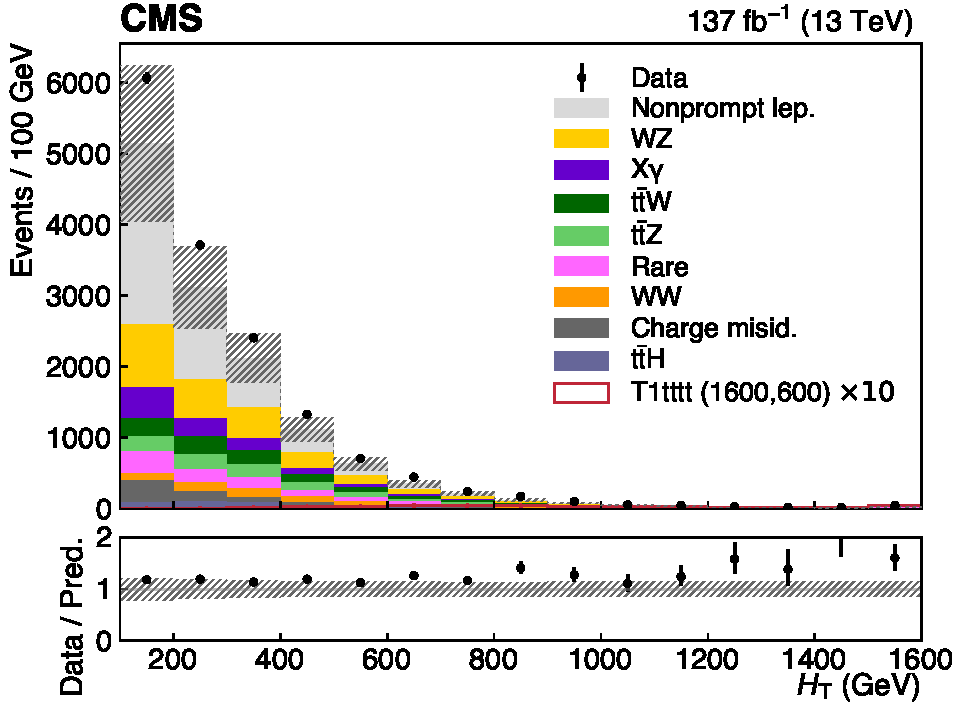
\includegraphics[width=.48\textwidth]{figs/ssp/br_ht.pdf}
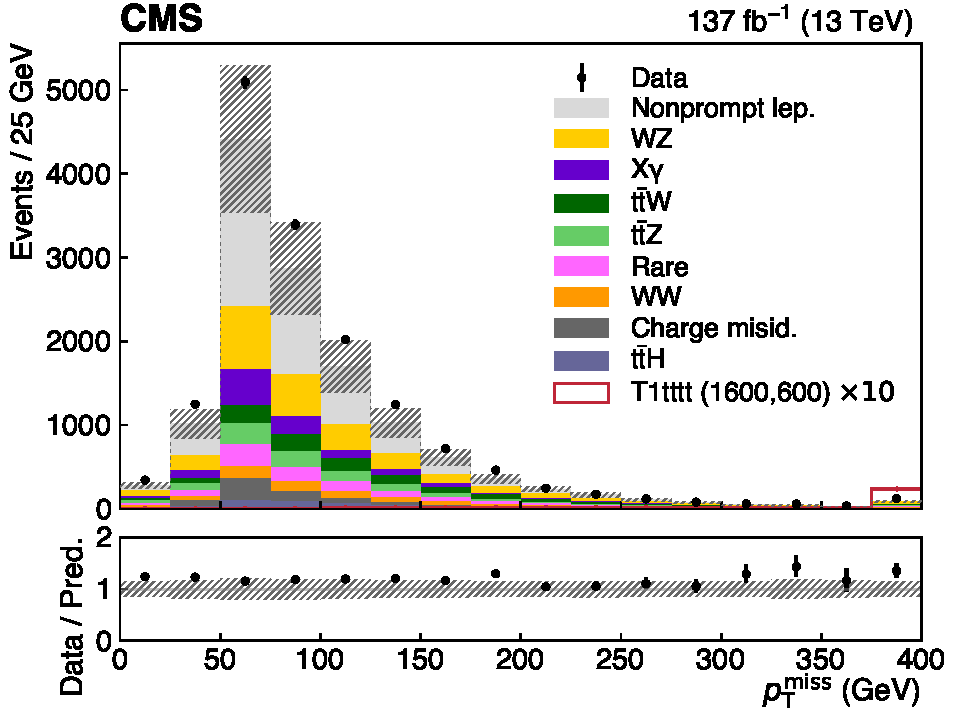
\includegraphics[width=.48\textwidth]{figs/ssp/br_met.pdf}
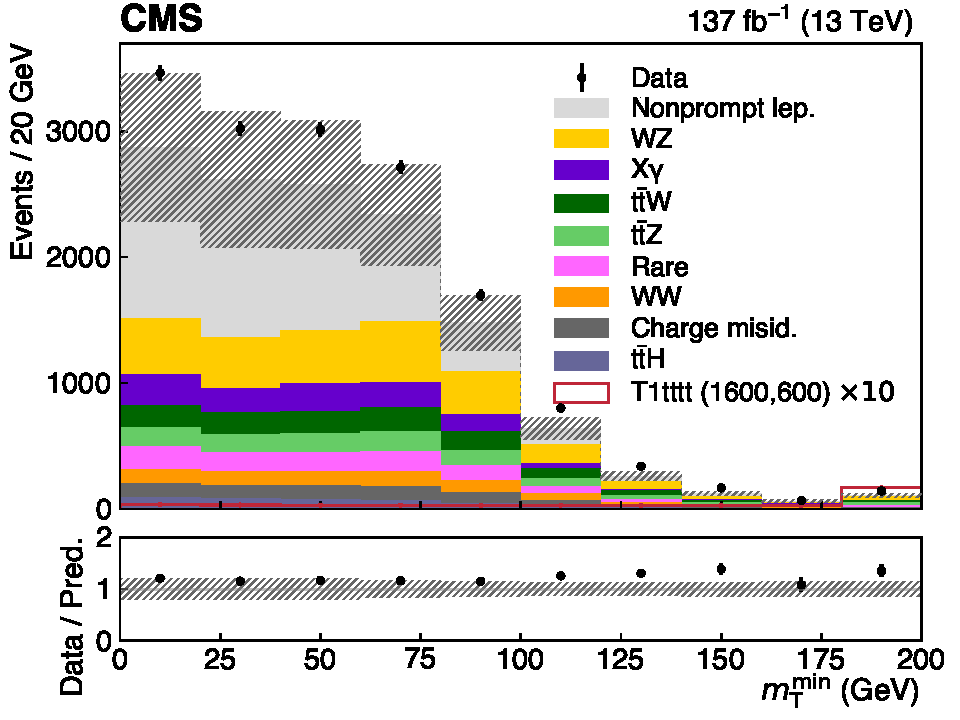
\includegraphics[width=.48\textwidth]{figs/ssp/br_mtmin.pdf}
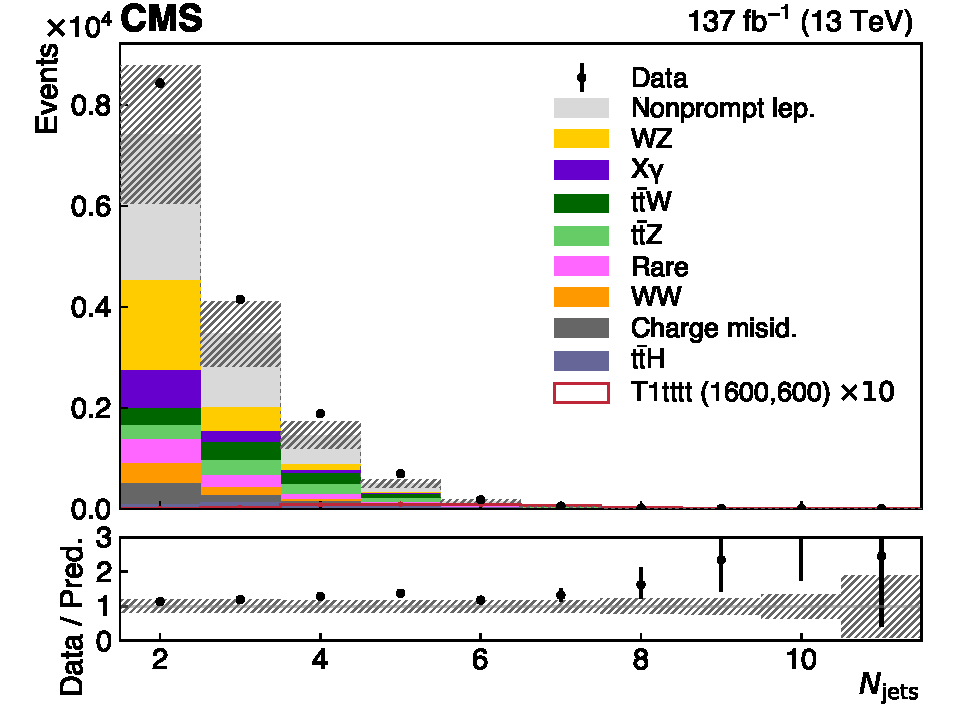
\includegraphics[width=.48\textwidth]{figs/ssp/br_njets.pdf}
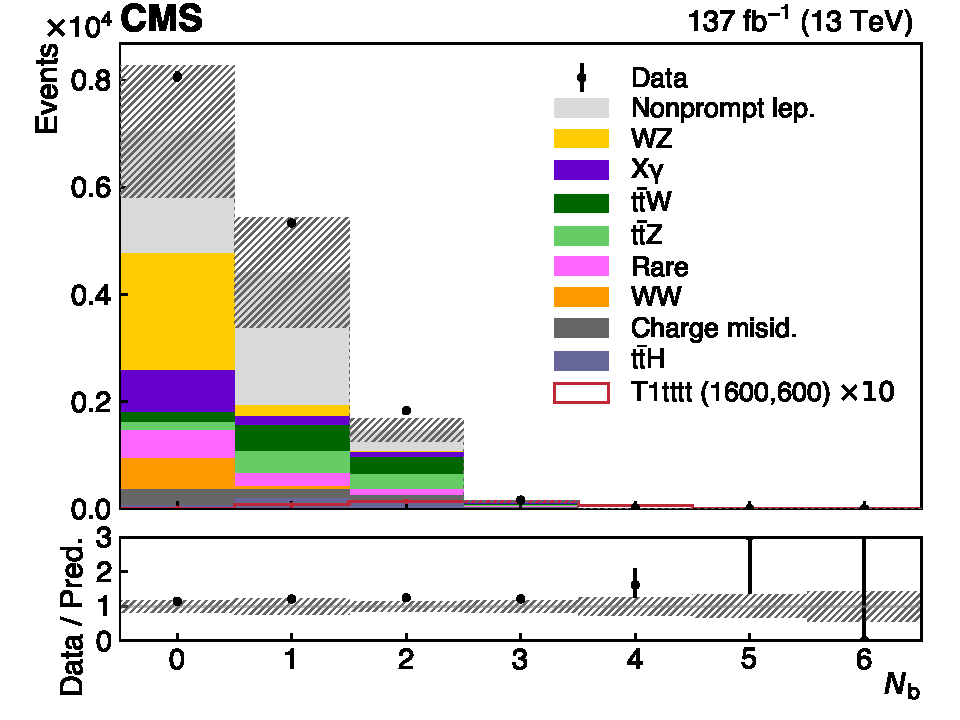
\includegraphics[width=.48\textwidth]{figs/ssp/br_nbtags.pdf}
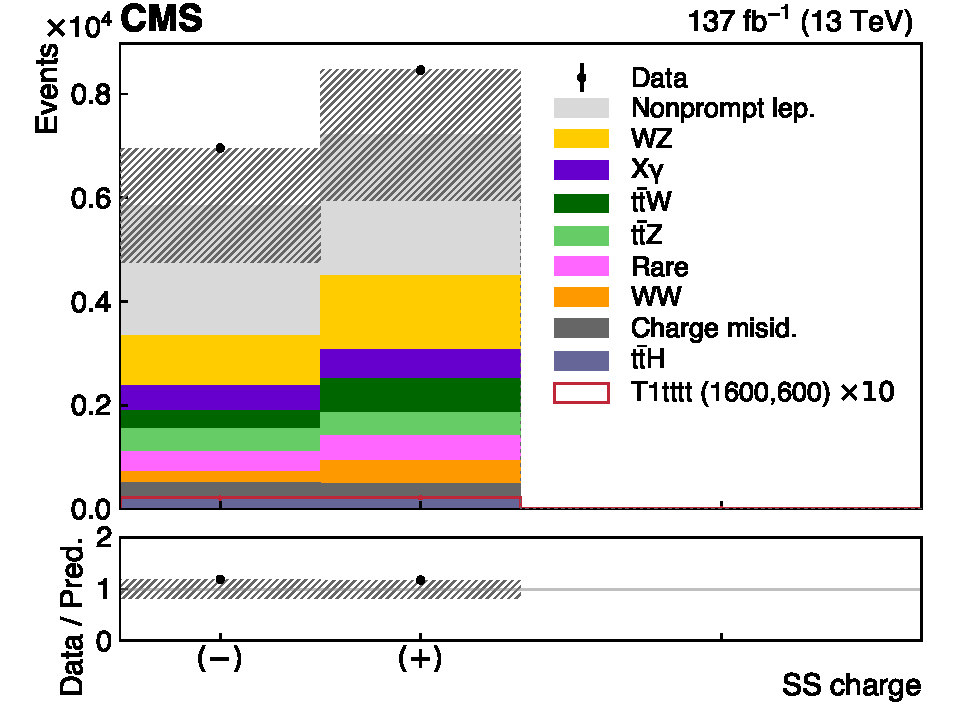
\includegraphics[width=.48\textwidth]{figs/ssp/br_charge.pdf}
\\
\caption{Distributions of the main analysis variables after the event selection:
\HT, \ptmiss, \MTmin, \Njets, \Nbjets, and the charge of the SS pair,
    where the last bin includes the overflow (where applicable). The hatched area represents the total statistical and systematic uncertainty in the background prediction.
The lower panels show the ratio of the observed event yield to the background prediction.
The prediction for the SUSY model \Totttt with $m_{\gluino}=1600\GeV$ and $m_{\lsp}=600\GeV$ is overlaid.
}
\label{fig:kinem}
\end{figure*}

\begin{figure*}[!hbtp]
\centering
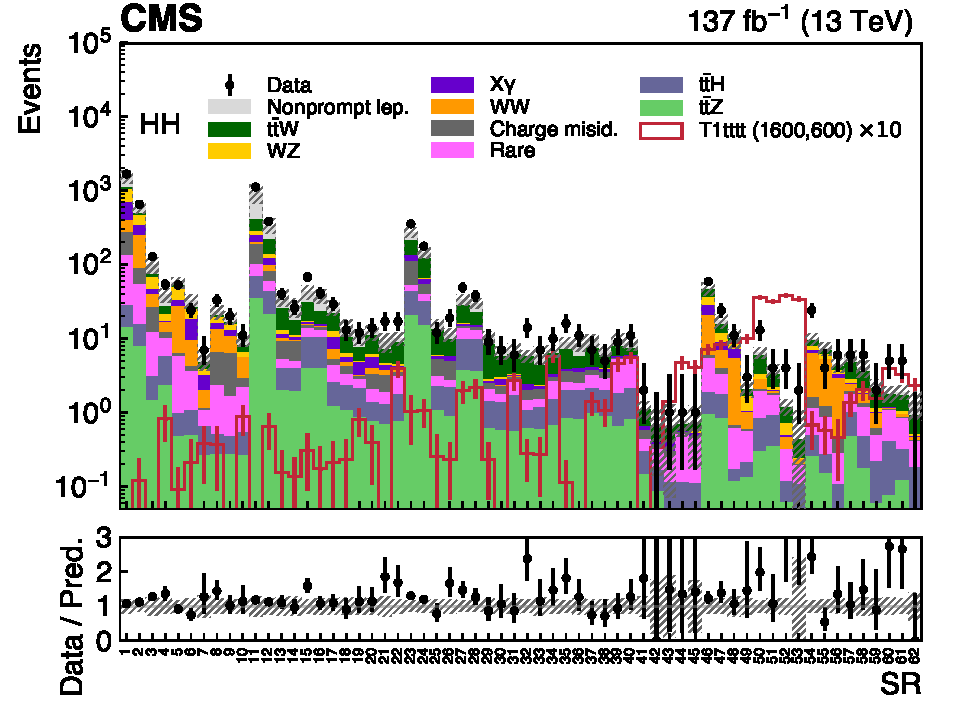
\includegraphics[width=.50\textwidth]{figs/ssp/SRHH_TOTAL.pdf}
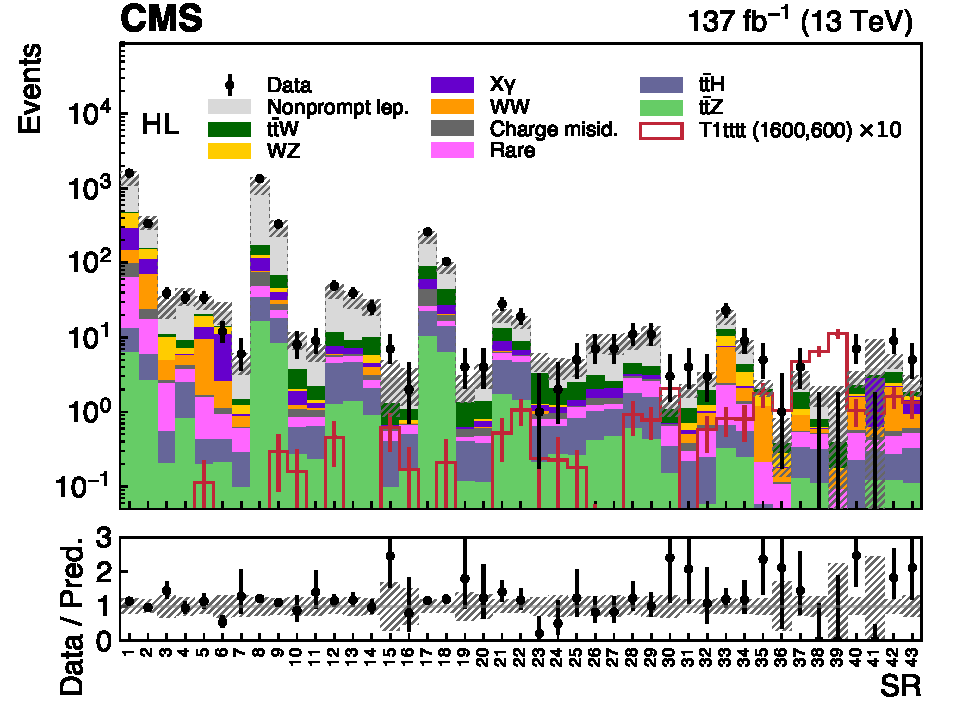
\includegraphics[width=.50\textwidth]{figs/ssp/SRHL_TOTAL.pdf}
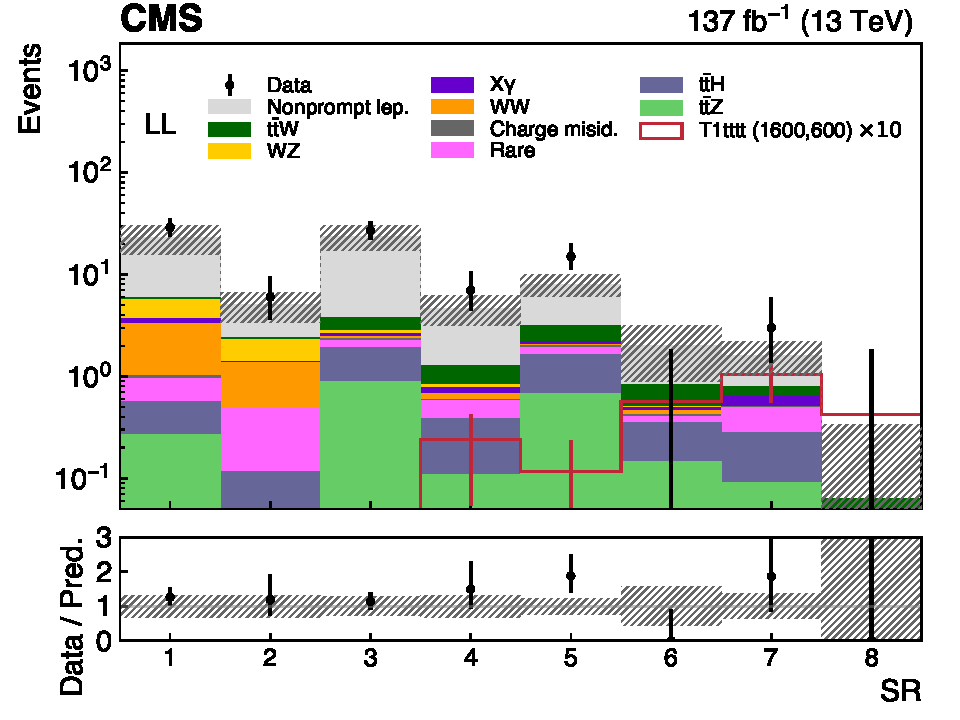
\includegraphics[width=.50\textwidth]{figs/ssp/SRLL_TOTAL.pdf}
\\
\caption{Expected and observed SR yields for the HH, HL, LL signal categories.
The hatched area represents the total statistical and systematic uncertainty in the background prediction.
}
\label{fig:SRrun2}
\end{figure*}

\begin{figure*}[!hbtp]
\centering
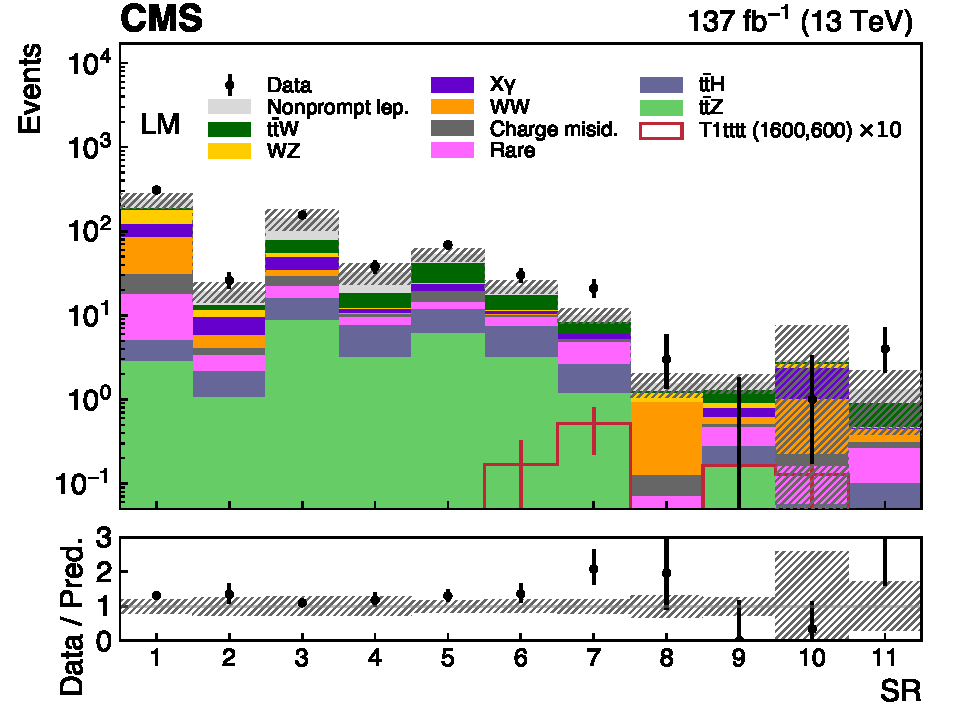
\includegraphics[width=.50\textwidth]{figs/ssp/SRLM_TOTAL.pdf}
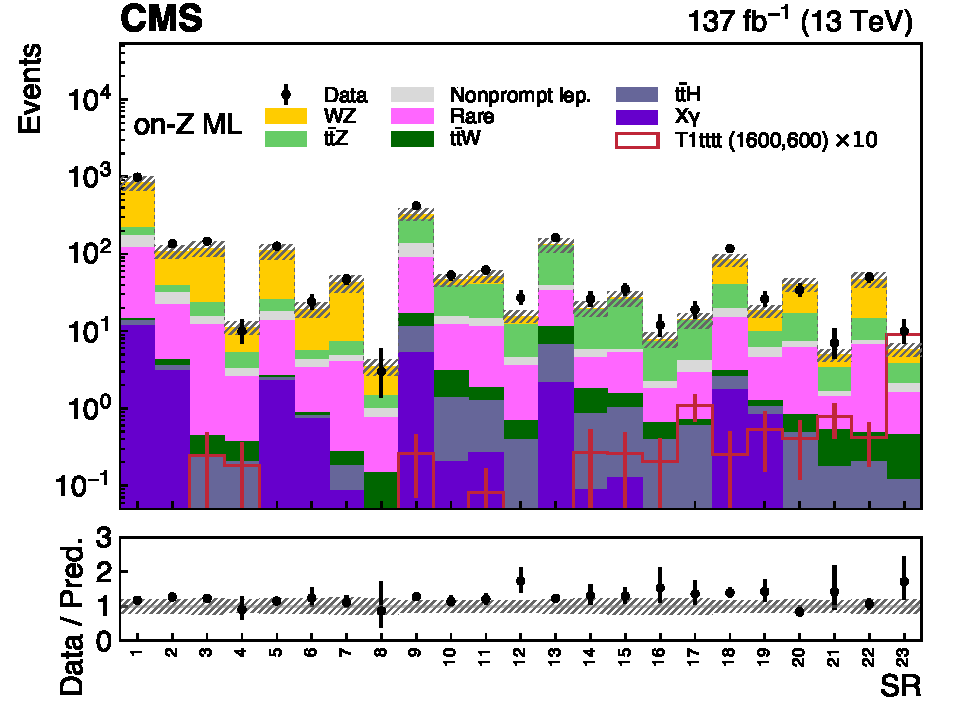
\includegraphics[width=.50\textwidth]{figs/ssp/SRMLONZ_TOTAL.pdf}
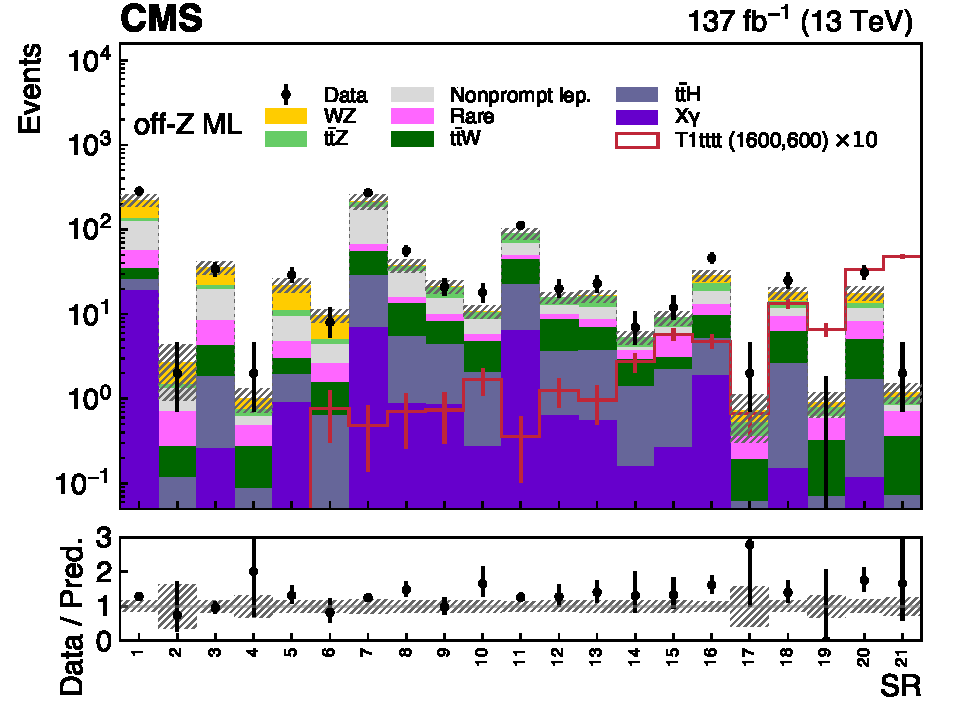
\includegraphics[width=.50\textwidth]{figs/ssp/SRMLOFFZ_TOTAL.pdf}
\\
\caption{Expected and observed SR yields for the LM, on-\PZ ML, off-\PZ ML signal categories. 
The hatched area represents the total statistical and systematic uncertainty in the background prediction.
}
\label{fig:SRrun2b}
\end{figure*}

\begin{table*}[!hbtp]
\centering
\label{tab:slimyields}
\begin{scriptsizetabular}{ccc|ccc|ccc}
\hline
\multicolumn{3}{c|}{HH regions}    &    \multicolumn{3}{c|}{HL regions}    &    \multicolumn{3}{c}{LM regions} \\ \hline
 SR    &    Expected SM    &    Obs.    &
 SR    &    Expected SM    &    Obs.    &
 SR    &    Expected SM    &    Obs. \\
 \hline
1   &    $1560\pm300 $    &   1673   &   1   &   $1390\pm300 $    &   1593   &   1   &    $235\pm47 $    &    309 \\
2   &    $582\pm93 $    &   653   &   2   &   $348\pm67 $    &   337   &   2   &    $19.3\pm5.2 $    &    26 \\
3   &    $100\pm25 $    &   128   &   3   &   $26.9\pm8.8 $    &   39   &   3   &    $142\pm39 $    &    156 \\
4   &    $39.5\pm8.5 $    &   54   &   4   &   $35.9\pm9.1 $    &   34   &   4   &    $32.2\pm8.8 $    &    38 \\
5   &    $57.7\pm9.9 $    &   53   &   5   &   $29.8\pm6.0 $    &   34   &   5   &    $53.0\pm9.1 $    &    69 \\
6   &    $32.5\pm7.1 $    &   24   &   6   &   $22.2\pm7.2 $    &   12   &   6   &    $22.0\pm4.0 $    &    30 \\
7   &    $5.5\pm1.8 $    &   7   &   7   &   $4.7\pm1.4 $    &   6   &   7   &    $10.1\pm2.0 $    &    21 \\
8   &    $22.9\pm5.1 $    &   33   &   8   &   $1100\pm280 $    &   1342   &   8   &    $1.53\pm0.48 $    &    3 \\
9   &    $19.5\pm3.9 $    &   20   &   9   &   $299\pm71 $    &   330   &   9   &    $1.58\pm0.41 $    &    0 \\
10   &    $9.6\pm1.9 $    &   11   &   10   &   $9.1\pm2.3 $    &   8   &   10   &    $2.9\pm2.9 $    &    1 \\
11   &    $940\pm270 $    &   1115   &   11   &   $6.4\pm1.6 $    &   9   &   11   &    $1.31\pm0.93 $    &    4 \\
12   &    $340\pm81 $    &   384   &   12   &   $42.1\pm9.2 $    &   49   &       &      &    \\\cline{7-9}
13   &    $36.3\pm9.5 $    &   40   &   13   &   $33.0\pm8.4 $    &   39   &    \multicolumn{3}{c}{on-\PZ ML regions} \\\cline{7-9}
14   &    $26.8\pm7.4 $    &   26   &   14   &   $25.8\pm5.9 $    &   25   &    SR    &    Expected SM    &    Obs. \\\cline{7-9}
15   &    $42.7\pm8.6 $    &   68   &   15   &   $2.8\pm2.0 $    &   7   &   1   &    $840\pm170 $    &    985 \\
16   &    $37.9\pm8.6 $    &   41   &   16   &   $2.5\pm1.3 $    &   2   &   2   &    $107\pm21 $    &    136 \\
17   &    $26.5\pm6.2 $    &   29   &   17   &   $222\pm42 $    &   260   &   3   &    $119\pm27 $    &    146 \\
18   &    $14.3\pm3.6 $    &   13   &   18   &   $86\pm15 $    &   104   &   4   &    $11.1\pm2.1 $    &    10 \\
19   &    $10.6\pm2.5 $    &   12   &   19   &   $2.22\pm0.90 $    &   4   &   5   &    $109\pm24 $    &    126 \\
20   &    $12.3\pm2.9 $    &   14   &   20   &   $3.2\pm1.1 $    &   4   &   6   &    $19.3\pm4.1 $    &    24 \\
21   &    $9.2\pm2.7 $    &   17   &   21   &   $19.8\pm3.8 $    &   28   &   7   &    $42\pm10 $    &    47 \\
22   &    $10.1\pm2.1 $    &   17   &   22   &   $16.1\pm3.0 $    &   19   &   8   &    $3.47\pm0.84 $    &    3 \\
23   &    $272\pm43 $    &   354   &   23   &   $4.7\pm1.3 $    &   1   &   9   &    $327\pm54 $    &    419 \\
24   &    $147\pm25 $    &   177   &   24   &   $4.0\pm1.2 $    &   2   &   10   &    $46.5\pm8.4 $    &    53 \\
25   &    $15.3\pm2.9 $    &   12   &   25   &   $4.0\pm1.1 $    &   5   &   11   &    $51.3\pm9.1 $    &    62 \\
26   &    $11.4\pm2.4 $    &   19   &   26   &   $8.5\pm2.4 $    &   7   &   12   &    $15.6\pm2.8 $    &    27 \\
27   &    $33.4\pm5.4 $    &   49   &   27   &   $8.4\pm2.5 $    &   7   &   13   &    $131\pm27 $    &    162 \\
28   &    $30.1\pm4.9 $    &   38   &   28   &   $8.9\pm2.2 $    &   11   &   14   &    $19.9\pm4.3 $    &    26 \\
29   &    $10.4\pm2.2 $    &   9   &   29   &   $10.9\pm3.1 $    &   11   &   15   &    $26.9\pm6.1 $    &    35 \\
30   &    $6.6\pm1.3 $    &   7   &   30   &   $1.25\pm0.39 $    &   3   &   16   &    $7.8\pm1.8 $    &    12 \\
31   &    $6.9\pm1.5 $    &   6   &   31   &   $1.92\pm0.37 $    &   4   &   17   &    $14.0\pm3.1 $    &    19 \\
32   &    $5.9\pm1.1 $    &   14   &   32   &   $2.77\pm0.56 $    &   3   &   18   &    $84\pm15 $    &    117 \\
33   &    $6.1\pm1.6 $    &   7   &   33   &   $19.1\pm4.1 $    &   23   &   19   &    $18.2\pm3.3 $    &    26 \\
34   &    $6.8\pm1.3 $    &   10   &   34   &   $7.5\pm1.5 $    &   9   &   20   &    $40.4\pm7.6 $    &    34 \\
35   &    $8.8\pm1.5 $    &   16   &   35   &   $2.12\pm0.49 $    &   5   &   21   &    $4.92\pm0.88 $    &    7 \\
36   &    $8.7\pm2.0 $    &   11   &   36   &   $0.47\pm0.33 $    &   1   &   22   &    $46.9\pm9.9 $    &    50 \\
37   &    $9.4\pm1.9 $    &   7   &   37   &   $2.75\pm0.77 $    &   4   &   23   &    $5.8\pm1.2 $    &    10 \\
38   &    $7.0\pm1.3 $    &   5   &   38   &   $1.68\pm0.50 $    &   0   &      &      &    \\\cline{7-9}
39   &    $9.6\pm2.1 $    &   9   &   39   &   $0.97\pm0.97 $    &   0   &    \multicolumn{3}{c}{off-\PZ ML regions} \\\cline{7-9}
40   &    $8.6\pm1.7 $    &   11   &   40   &   $2.83\pm0.70 $    &   7   &    SR    &    Expected SM    &    Obs. \\\cline{7-9}
41   &    $1.10\pm0.32 $    &   2   &   41   &   $3.8\pm3.8 $    &   0   &   1   &    $222\pm36 $    &    285 \\
42   &    $0.63\pm0.49 $    &   0   &   42   &   $4.9\pm1.0 $    &   9   &   2   &    $2.7\pm1.7 $    &    2 \\
43   &    $0.67\pm0.60 $    &   1   &   43   &   $2.36\pm0.72 $    &   5   &   3   &    $35.5\pm6.4 $    &    34 \\
44   &    $0.74\pm0.27 $    &   1   &       &       &      &   4   &    $0.99\pm0.31 $    &    2 \\\cline{4-6}
45   &    $0.71\pm0.53 $    &   1   &    \multicolumn{3}{c|}{LL regions}                &   5   &    $22.1\pm4.0 $    &    29 \\\cline{4-6}
46   &    $47.8\pm9.7 $    &   59   &    SR    &    Expected SM    &    Obs.    &   6   &    $9.7\pm1.7 $    &    8 \\\cline{4-6}
47   &    $17.3\pm3.8 $    &   24   &   1   &    $23.0\pm7.2 $    &   29   &   7   &    $217\pm44 $    &    272 \\
48   &    $10.3\pm2.9 $    &   11   &   2   &    $5.0\pm1.6 $    &   6   &   8   &    $37.7\pm6.8 $    &    56 \\
49   &    $2.06\pm0.49 $    &   3   &   3   &    $23.8\pm6.6 $    &   27   &   9   &    $21.4\pm3.7 $    &    21 \\
50   &    $6.5\pm1.1 $    &   13   &   4   &    $4.7\pm1.5 $    &   7   &   10   &    $10.9\pm1.9 $    &    18 \\
51   &    $3.72\pm0.79 $    &   4   &   5   &    $8.0\pm1.9 $    &   15   &   11   &    $89\pm14 $    &    112 \\
52   &    $1.21\pm0.29 $    &   4   &   6   &    $2.0\pm1.1 $    &   0   &   12   &    $15.6\pm2.4 $    &    20 \\
53   &    $0.44\pm0.44 $    &   2   &   7   &    $1.61\pm0.59 $    &   3   &   13   &    $16.4\pm2.7 $    &    23 \\
54   &    $9.8\pm1.8 $    &   24   &   8   &    $0.06\pm0.06 $    &   0   &   14   &    $5.36\pm0.95 $    &    7 \\
55   &    $7.3\pm1.4 $    &   4   &       &       &      &   15   &    $9.0\pm1.6 $    &    12 \\
56   &    $4.44\pm0.98 $    &   6   &       &       &      &   16   &    $28.4\pm3.9 $    &    46 \\
57   &    $5.7\pm1.1 $    &   6   &       &       &      &   17   &    $0.72\pm0.41 $    &    2 \\
58   &    $4.0\pm1.0 $    &   6   &       &       &      &   18   &    $17.8\pm2.8 $    &    25 \\
59   &    $2.24\pm0.53 $    &   2   &       &       &      &   19   &    $0.89\pm0.29 $    &    0 \\
60   &    $1.83\pm0.44 $    &   5   &       &       &      &   20   &    $17.7\pm3.3 $    &    31 \\
61   &    $1.88\pm0.40 $    &   5   &       &       &      &   21   &    $1.20\pm0.32 $    &    2 \\
62   &    $1.35\pm0.56 $    &   0   &       &       &      &      &      &   \\
\hline
\end{scriptsizetabular}
\caption{
Expected background event yields, total uncertainties, and observed event yields in the SRs used in this search.
}
\end{table*}

                               
\FloatBarrier

\section{SUSY interpretations}
\label{sec:ssinterpretations}

\subsection{Model-dependent}

The results are interpreted as constraints on the cross sections for signal
models. Event yields in all SRs are used to obtain exclusion limits on the
production cross section of each model at 95\% confidence level (\CL) with an
asymptotic formulation of the modified frequentist \CLs
criterion~\cite{STAT:Junk1999kv,STAT:Read2002hq,STAT:ATLPHYSPUB2011011,STAT:Cowan2010js},
where uncertainties are incorporated as nuisance parameters and
profiled~\cite{STAT:ATLPHYSPUB2011011}. Since the normalizations of the
various backgrounds allowed to vary within their uncertainties in the
likelihood fit, several backgrounds (nonprompt lepton, $\ttbar \PW/\PZ/\PH$
and rare processes) are pulled up by around $1$ s.d. This is consistent with
the latest measurements of $\ttbar \PW$ and $\ttbar \PZ$ processes performed
by the ATLAS and CMS Collaborations~\cite{ATLAS:ttV,CMS:ttV}.


Figure~\ref{fig:t1ttxx_scan_xsec} shows observed and expected exclusion
limits for simplified models of gluino pair production with each gluino
decaying to off- or on-shell third-generation squarks, \Totttt, \TfttbbWW,
\Tftttt, and \Tfttcc. Figs.~\ref{fig:t5qqqqvv_scan_xsec}
and~\ref{fig:t5qqqqww_scan_xsec} show the corresponding limits for \TfqqqqWZ
and \TfqqqqWW, with two different assumptions on the chargino mass. The
\TfqqqqWZ model assumes equal probabilities for the decay of the gluino into
\chiplus, \chiminus, and \neutralinotwo. The exclusion limits for \TsttWW and
\TsttHZ are displayed in Figs.~\ref{fig:t6ttww_scan_xsec}
and~\ref{fig:t6tthz_scan_xsec}, respectively. The three sets of exclusion
limits shown in Fig.~\ref{fig:t6tthz_scan_xsec} correspond to the branching
fraction $\mathcal{B}(\susytoptwo\to\susytopone\PZ)$ having values of 0, 50,
and 100\%.

For the RPV models, Fig.~\ref{fig:rpvlimits} 
shows observed and expected limits on the
cross section of gluino pair production as a function of the gluino masses.
Both the observed and expected exclusions on the gluino mass
are similar and reach 2.1 and 1.7 \TeV for the \ToqqqqL and \Totbs models,
respectively.

As there are many SRs and many topologically diverse signal models,
it can be hard to associate sensitivity and performance with particular
SRs or kinematic categories. To help with this,
Table~\ref{tab:toprankedSRs} presents the top five SRs for several
representative models, ranked based on the largest values of
$N_\text{sig.}/\sqrt{N_\text{bkg.} + N_\text{sig.}}$, where $N_\text{sig.}$
and $N_\text{bkg.}$ are the signal and total background yields in each SR,
respectively. At a glance, one sees that high $\ptmiss$ and high $\HT$ regions
in the HH kinematic category provide sensitivity for many high mass splitting
topologies, while the LL category provides sensitivity for more compressed
topologies.

\begin{table}
\footnotesize
\begin{center}
    \caption{
        Top five SRs for several representative models, ranked based on the largest values of $N_\text{sig.}/\sqrt{N_\text{bkg.} + N_\text{sig.}}$,
    where $N_\text{sig.}$ and $N_\text{bkg.}$ are the signal and total background yields in each SR, respectively.
    }
\label{tab:toprankedSRs}
\resizebox{0.99\textwidth}{!}{
{\renewcommand{\arraystretch}{1.6}
\begin{tabular}{ccc}\hline
model      & mass point   & top SRs \\
\hline
\Totttt                                               & $m_{\gluino}=1400, m_{\lsp}=400$           & off-Z ML21, HH53, HH52, HH51, HH50 \\
\Totttt                                               & $m_{\gluino}=2000, m_{\lsp}=100$           & HH53, HH52, off-Z ML21, HL39, HH49 \\
\Totttt                                               & $m_{\gluino}=1800, m_{\lsp}=100$           & HH53, off-Z ML21, HH52, HL39, HH51 \\
\Totttt                                               & $m_{\gluino}=1800, m_{\lsp}=1000$          & off-Z ML21, HH53, HH52, HH51, HH50 \\
\Totttt                                               & $m_{\gluino}=1800, m_{\lsp}=1550$          & HH53, HL39, off-Z ML21, HH49, HH52 \\
\TsttWW                                               & $m_{\sbottomone}=1000, m_{\chiplmin}=600$  & off-Z ML21, HH53, HH51, HH50, HH52 \\
\TsttWW                                               & $m_{\sbottomone}=900, m_{\chiplmin}=400$   & off-Z ML21, HH51, HH50, HH53, off-Z ML20 \\
\TsttWW                                               & $m_{\sbottomone}=800, m_{\chiplmin}=400$   & off-Z ML21, HH51, HH50, HH34, off-Z ML20 \\
\TfqqqqWZ                                             & $m_{\gluino}=1400, m_{\lsp}=1$             & on-Z ML23, HH53, HH52, HH51, HH49 \\
\TfqqqqWZ                                             & $m_{\gluino}=900, m_{\lsp}=600$            & on-Z ML4, HH3, HH10, on-Z ML23, HH4 \\
\TfqqqqWW                                             & $m_{\gluino}=1400, m_{\lsp}=1$             & HH53, HH52, HH49, HH51, HH50 \\
\TfqqqqWW                                             & $m_{\gluino}=900, m_{\lsp}=600$            & HH3, HH10, HH4, HH7, HH50 \\
\TfqqqqWZ ($m_{\chiplmin} = m_{\lsp} + 20\GeV$)       & $m_{\gluino}=1400, m_{\lsp}=1$             & HH59, HH53, HH52, HH62, HH51 \\
\TfqqqqWZ ($m_{\chiplmin} = m_{\lsp} + 20\GeV$)       & $m_{\gluino}=900, m_{\lsp}=600$            & LL2, LL1, LL4, HL39, HL37 \\
\TfqqqqWW ($m_{\chiplmin} = m_{\lsp} + 20\GeV$)       & $m_{\gluino}=1400, m_{\lsp}=1$             & HH59, HH53, HH52, HH51, HH62 \\
\TfqqqqWW ($m_{\chiplmin} = m_{\lsp} + 20\GeV$)       & $m_{\gluino}=900, m_{\lsp}=600$            & LL2, LL4, HL39, LL1, HL37 \\
\TsttHZ ($\mathcal{B}(\susytoptwo\to\susytopone\PZ)$=1) & $m_{\susytoptwo}=850, m_{\susytopone}=625$ & on-Z ML23, on-Z ML21, on-Z ML16, on-Z ML14, on-Z ML17 \\
\TsttHZ ($\mathcal{B}(\susytoptwo\to\susytopone\PZ)$=0.5) & $m_{\susytoptwo}=850, m_{\susytopone}=625$ & on-Z ML17, on-Z ML23, on-Z ML21, on-Z ML14, on-Z ML16 \\
\TsttHZ ($\mathcal{B}(\susytoptwo\to\susytopone\PZ)$=0) & $m_{\susytoptwo}=850, m_{\susytopone}=625$ & off-Z ML15, HH40, HH39, HH45, HH44 \\
\ToqqqqL                                              & $m_{\gluino}=1600$                         & HH62, LM11, HH59, HH61, HH51 \\
\ToqqqqL                                              & $m_{\gluino}=2400$                         & HH62, LM11, HH59, HH53, HH52 \\
\Totbs                                                & $m_{\gluino}=1200$                         & HH62, HH50, HH59, HH61, HH58 \\
\Totbs                                                & $m_{\gluino}=1700$                         & HH62, HH59, HH50, HH52, LM11 \\
\hline
\end{tabular}}}
\end{center}
\end{table}

% The analysis sensitivity for the various models studied in
% Figs.~\ref{fig:t1ttxx_scan_xsec}--\ref{fig:t6tthz_scan_xsec} is often driven
% by the event yields in a few SRs (off-\PZ ML21, HH53 and HH52), where a
% slight excess of data is observed. This in particular applies to the
% uncompressed mass regime, resulting in an observed limit weaker than the
% expected one by one or two s.d. In the compressed mass regime, however, other
% SRs can become dominant, for example when the hadronic activity becomes
% limited. This happens in the \TfqqqqWZ and \TfqqqqWW models where the gluino
% and the lightest neutralino present a limited mass splitting (the region
% close to the diagonal in the left plots of Figs.~\ref{fig:t5qqqqvv_scan_xsec}
% and ~\ref{fig:t5qqqqww_scan_xsec}). In those scenarios the on-\PZ ML4 and HH3
% SRs provide the best sensitivity, respectively. Additionally, if the
% intermediate chargino is nearly degenerate in mass with the lightest
% neutralino, both leptons become soft and LL SRs such as LL2 become relevant.
% Such a situation is encountered in the phase space region close to the
% diagonal in the right plots of Figs.~\ref{fig:t5qqqqvv_scan_xsec} and
% ~\ref{fig:t5qqqqww_scan_xsec}. On-\PZ SRs (especially on-\PZ ML23) become
% important for models where an on-shell \PZ boson is produced (bottom plot in
% Fig.~\ref{fig:t6tthz_scan_xsec}). The limits on the RPV models presented in
% Fig.~\ref{fig:rpvlimits} are mostly driven by another set of SRs (HH62 and
% LM11, the latter becoming more relevant for lower masses).


Compared to previous versions of this
analysis~\cite{CMS:mySUS2016,CMS:SUS16041}, limits for the RPC models extend
the gluino and squark mass observed and expected exclusions by up to 200\GeV
primarily due to the increase in the integrated luminosity
($35.9\rightarrow\mathrm{\sslumi}$) and the corresponding re-optimization of
SR definitions. These results also complement searches for gluino pair
production conducted by CMS in final states with 0 or 1
lepton~\cite{CMS:2019tlp,CMS:Sirunyan2019ctn,CMS:Sirunyan2019xwh}. The
constraints on the two RPV models that were not previously included
demonstrate the sensitivity of the analysis to RPV scenarios. The final state
is particularly well suited to study the \ToqqqqL model as there is no
penalty from leptonic branching fraction, which results in exclusion limits
on the gluino mass beyond 2.1 \TeV, comparable to other results in fully
hadronic final states~\cite{CMS:Sirunyan2019ctn,CMS:Sirunyan2019xwh}. The
limits obtained on the \Totbs model are stronger than those previously
obtained in the one-lepton channel based on the analysis of the 2016
dataset~\cite{CMS:Sirunyan2017dhe}.

\begin{figure*}[!hbtp]
\centering
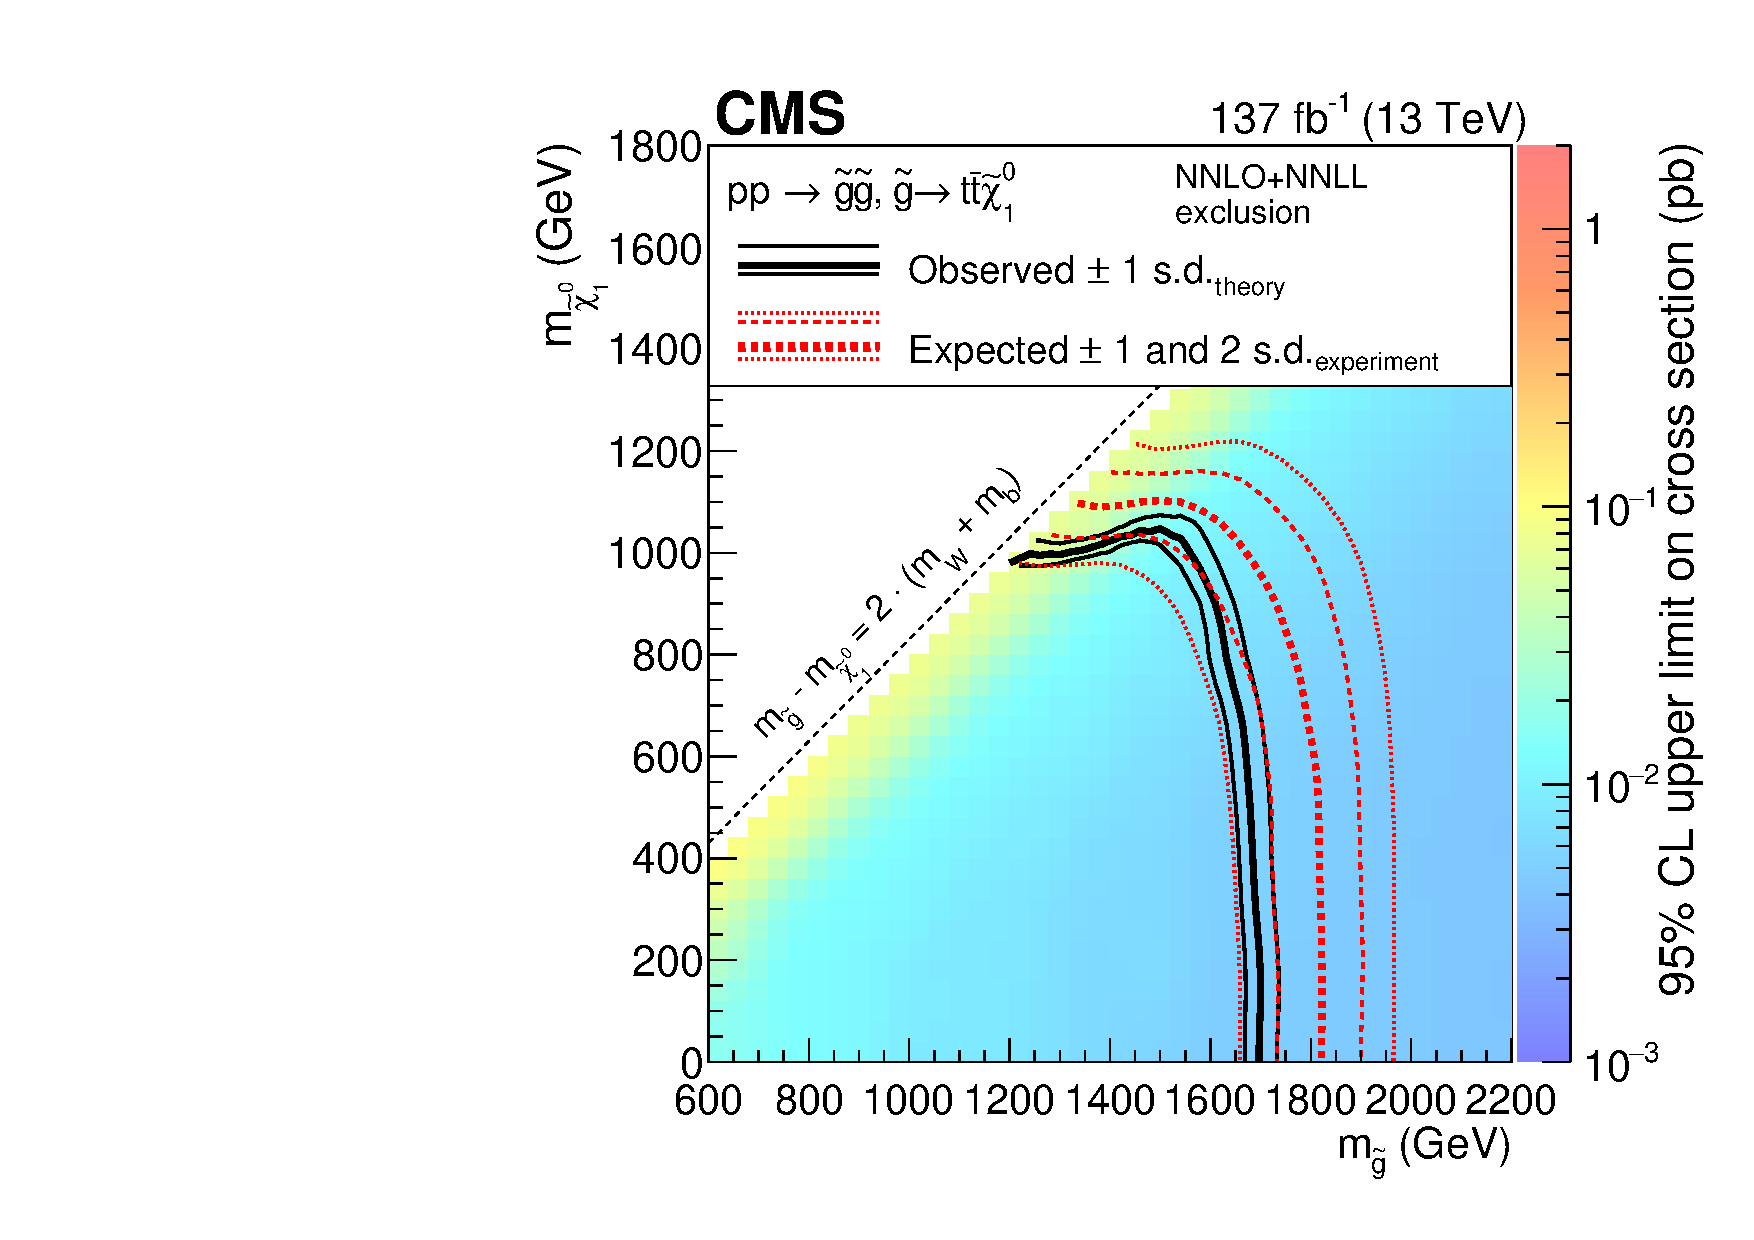
\includegraphics[width=0.45\textwidth]{figs/ssp/scan_t1tttt.pdf}
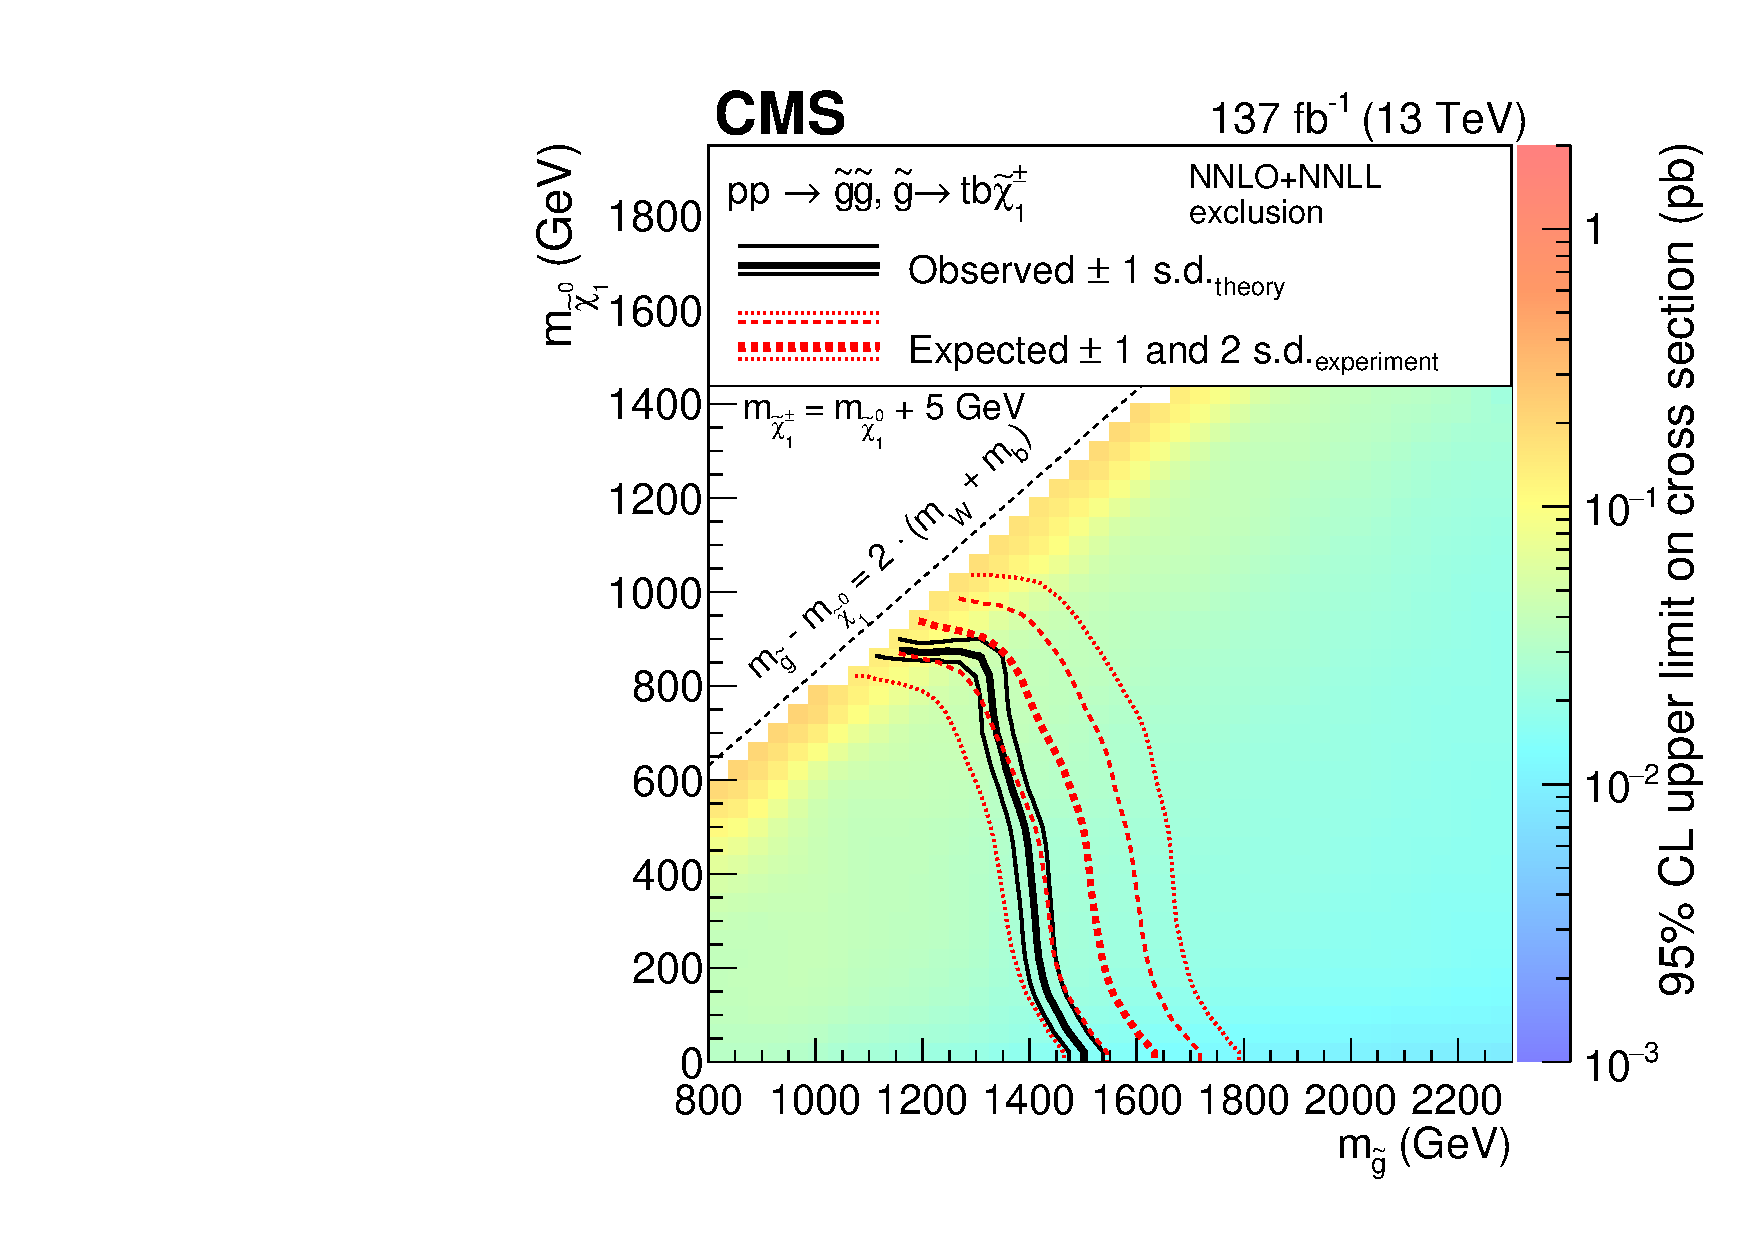
\includegraphics[width=0.45\textwidth]{figs/ssp/scan_t1ttbb.pdf}
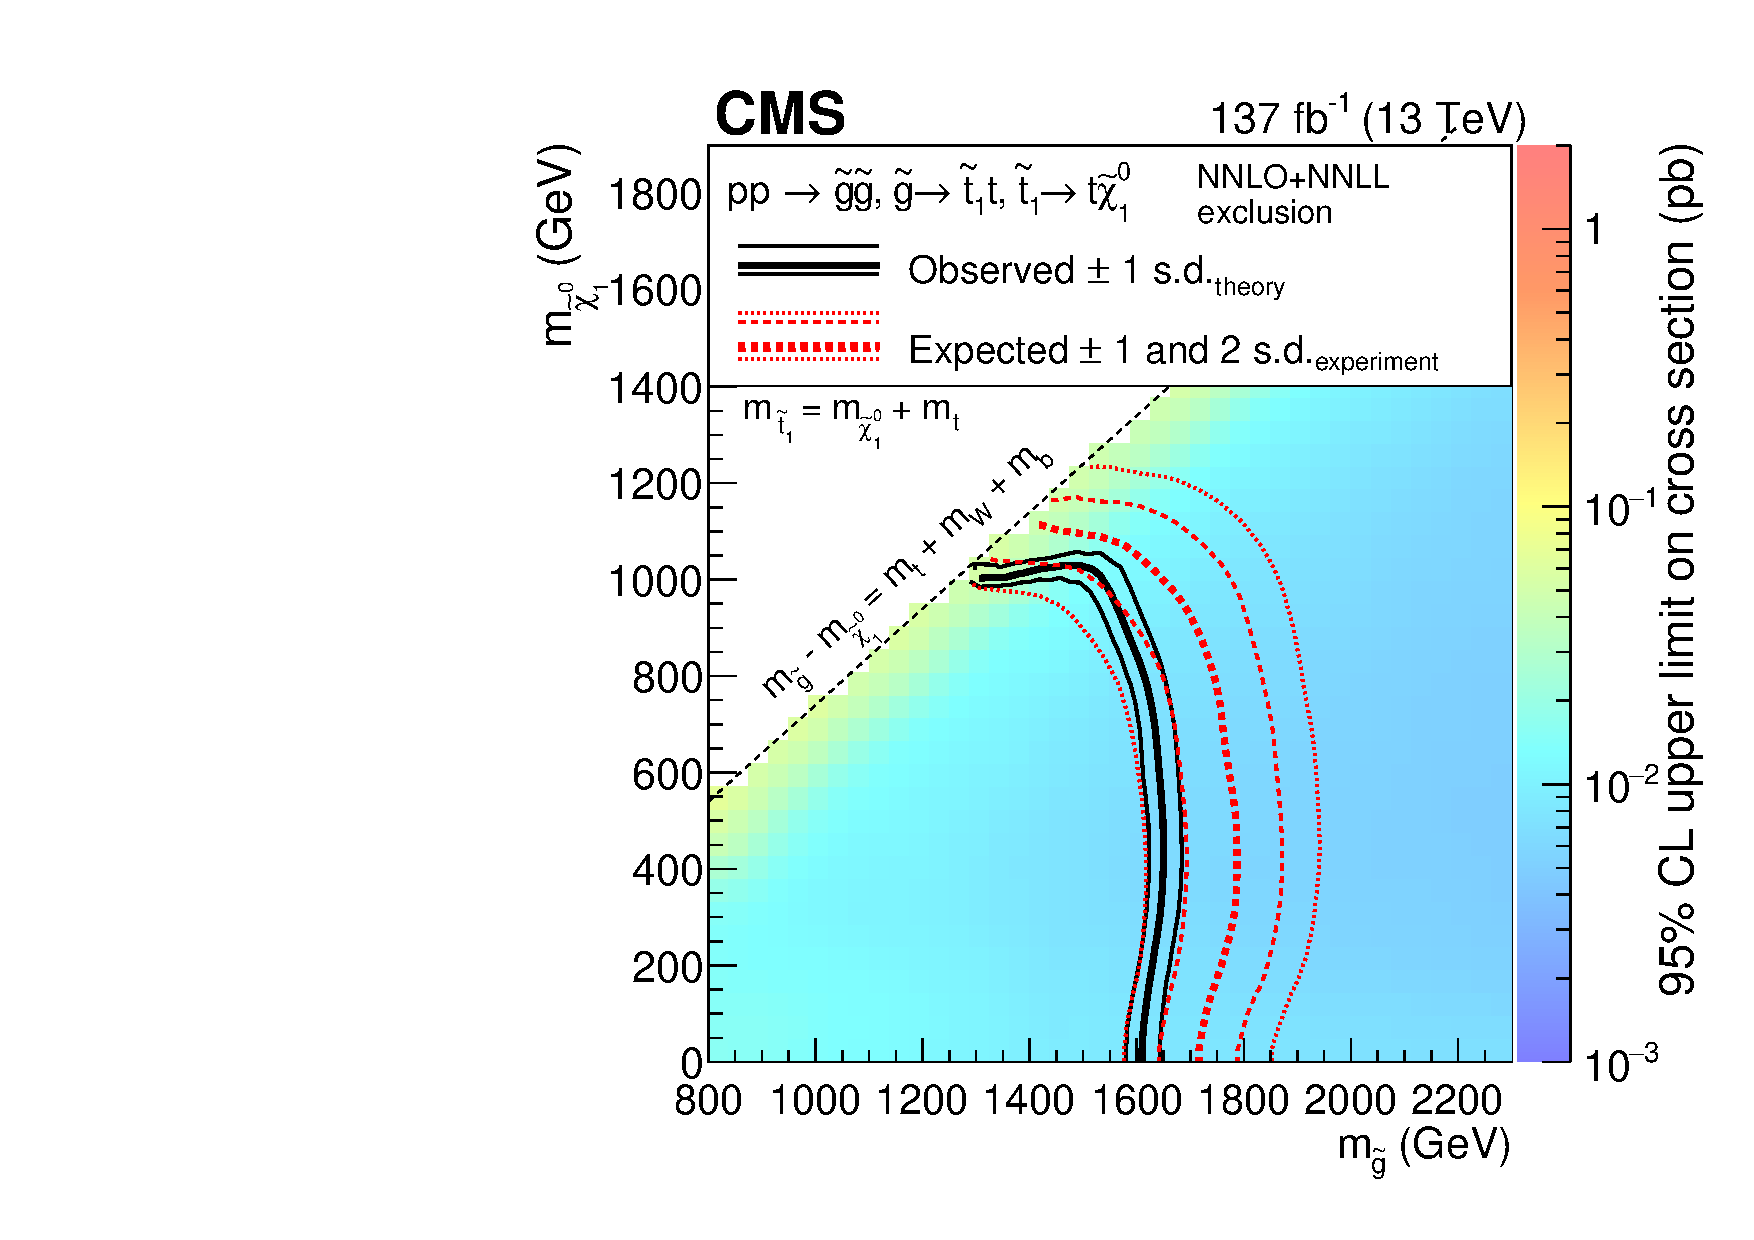
\includegraphics[width=0.45\textwidth]{figs/ssp/scan_t5tttt.pdf}
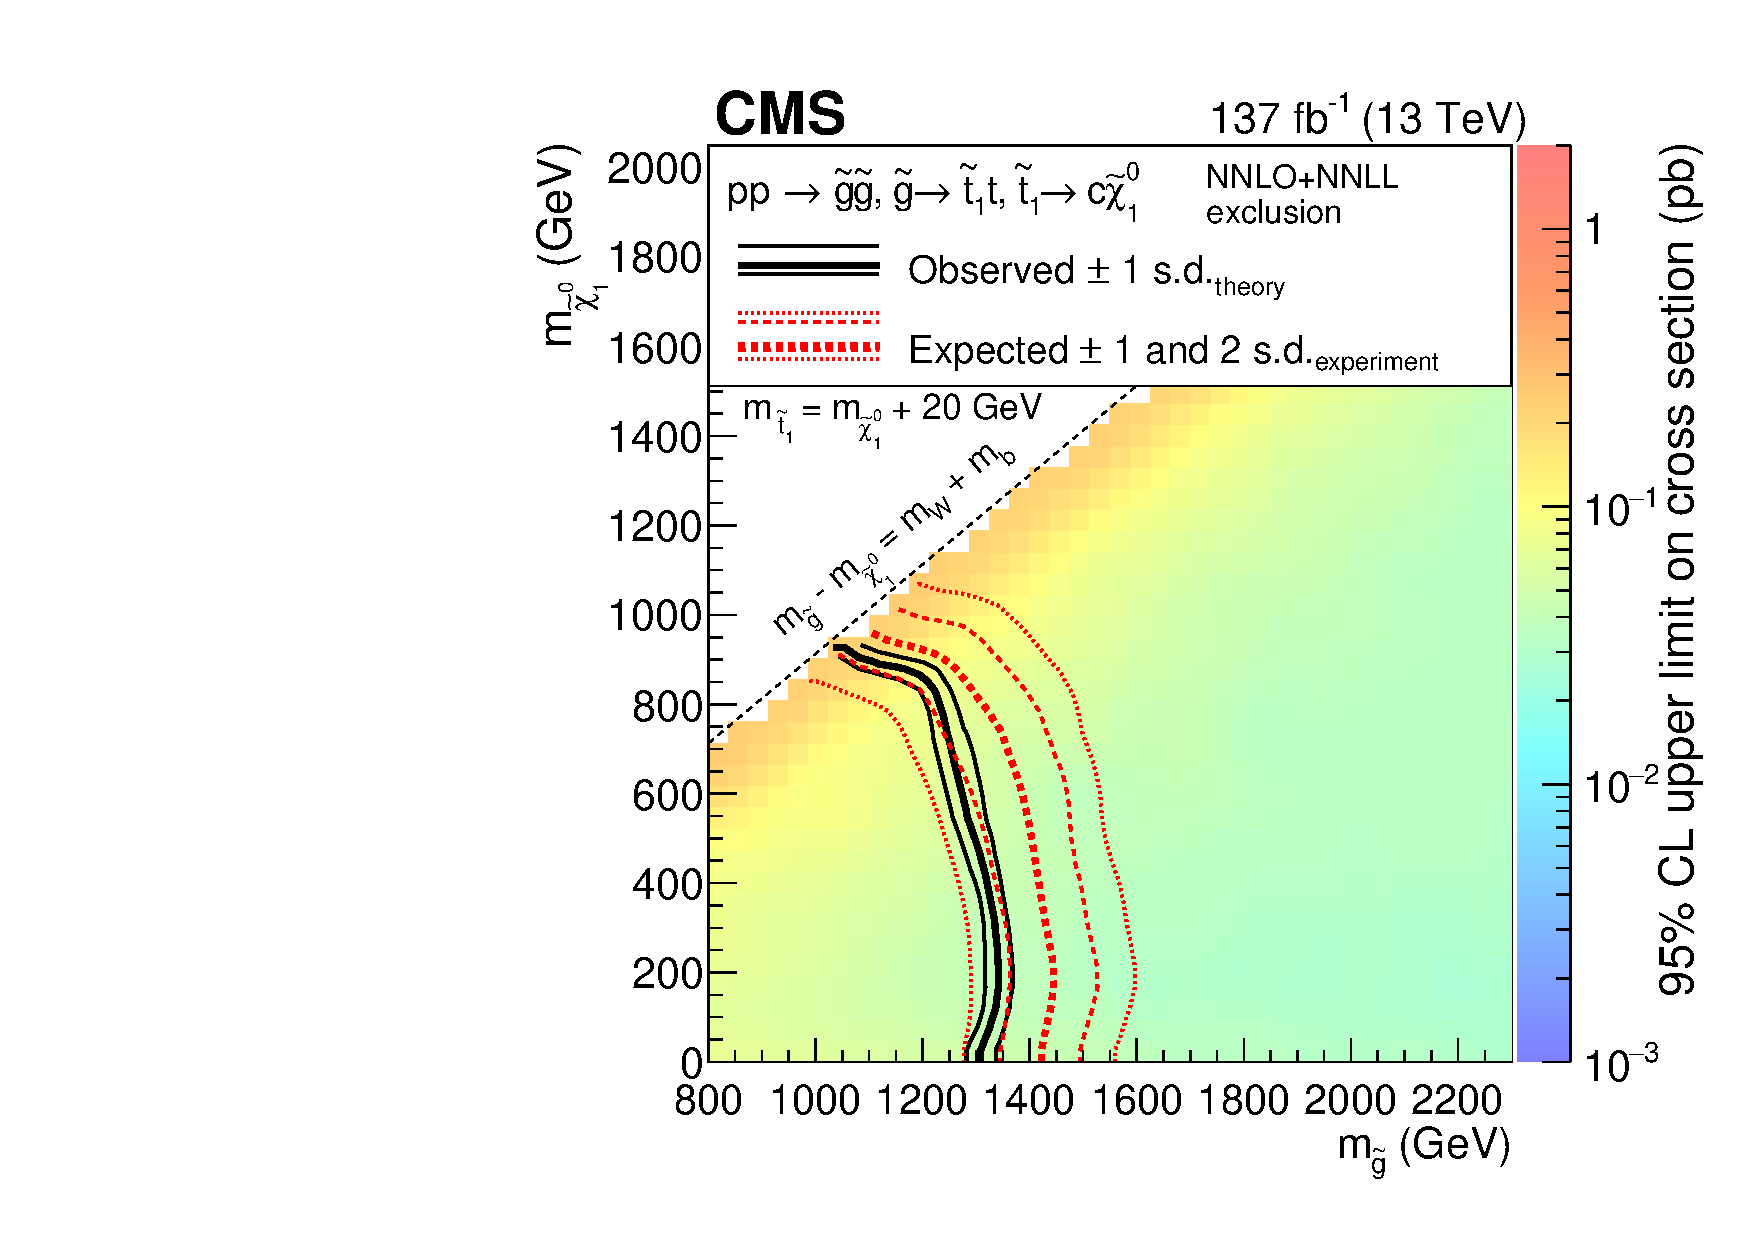
\includegraphics[width=0.45\textwidth]{figs/ssp/scan_t5ttcc.pdf}
\caption{ Exclusion regions at 95\% \CL in the $m_{\lsp}$ versus
  $m_{\gluino}$ plane for the \Totttt~(upper left) and \TfttbbWW~(upper right) models, with off-shell third-generation squarks, and the
    \Tftttt~(lower left) and \Tfttcc (lower right) models, with on-shell third-generation squarks.
For the \TfttbbWW model, $m_{\chiplmin} = m_{\lsp} + 5\GeV$, for the \Tftttt model, $m_{\susytop} - m_{\lsp} = m_{\PQt}$, and
for the \Tfttcc model, $m_{\susytop} - m_{\lsp} = 20\GeV$ and the decay proceeds through $\susytop \to \PQc \lsp$.
The right-hand side color scale indicates the excluded cross section values for a given point in the SUSY particle mass plane.
The solid black curves represent the observed exclusion limits
assuming the approximate-NNLO+NNLL cross sections
(thick line), or their variations of $\pm 1$ standard deviations (s.d.) (thin lines).
The dashed red curves show the expected limits with the corresponding $\pm 1$ s.d. and $\pm 2$ s.d. uncertainties.
Excluded regions are to the left and below the limit curves.
}
\label{fig:t1ttxx_scan_xsec}
\end{figure*}

\begin{figure*}[!hbtp]
\centering
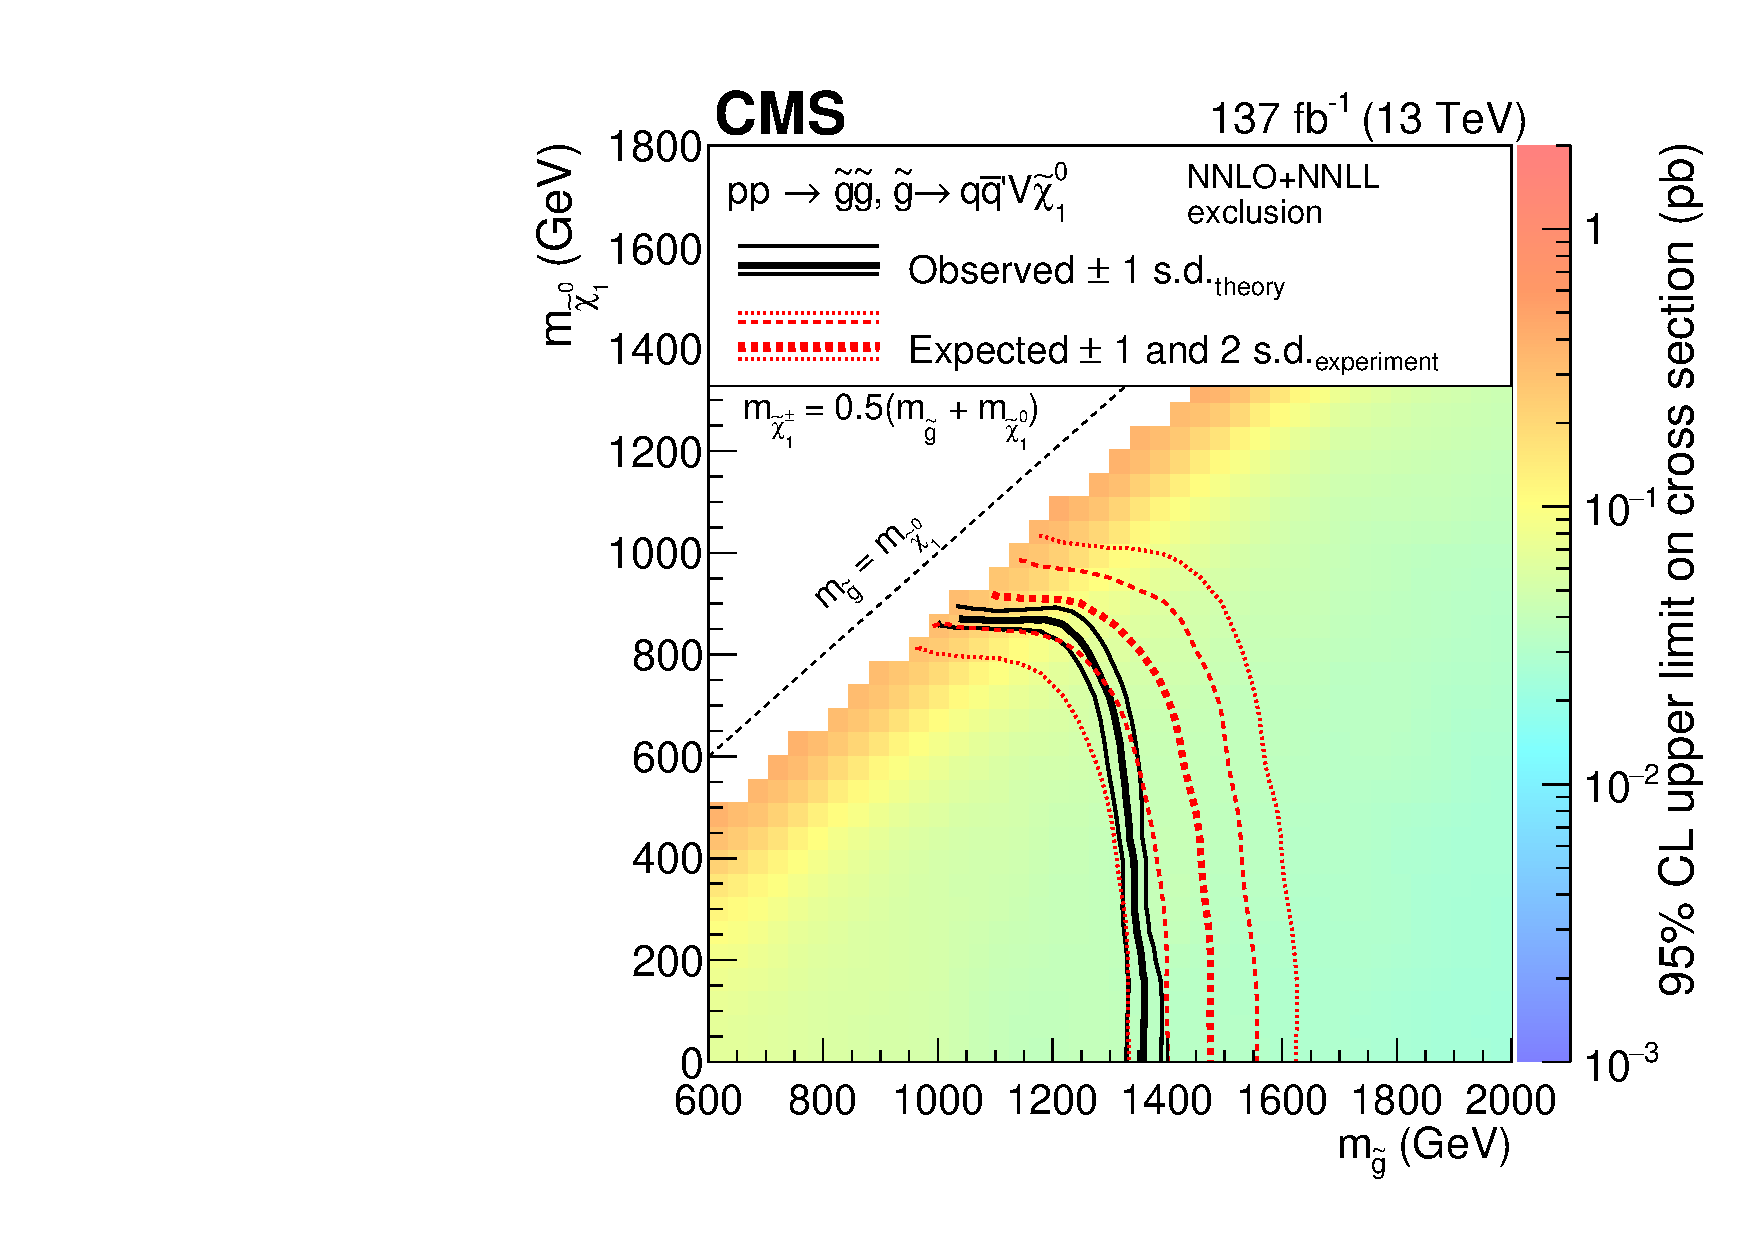
\includegraphics[width=0.45\textwidth]{figs/ssp/scan_t5qqqqvv.pdf}
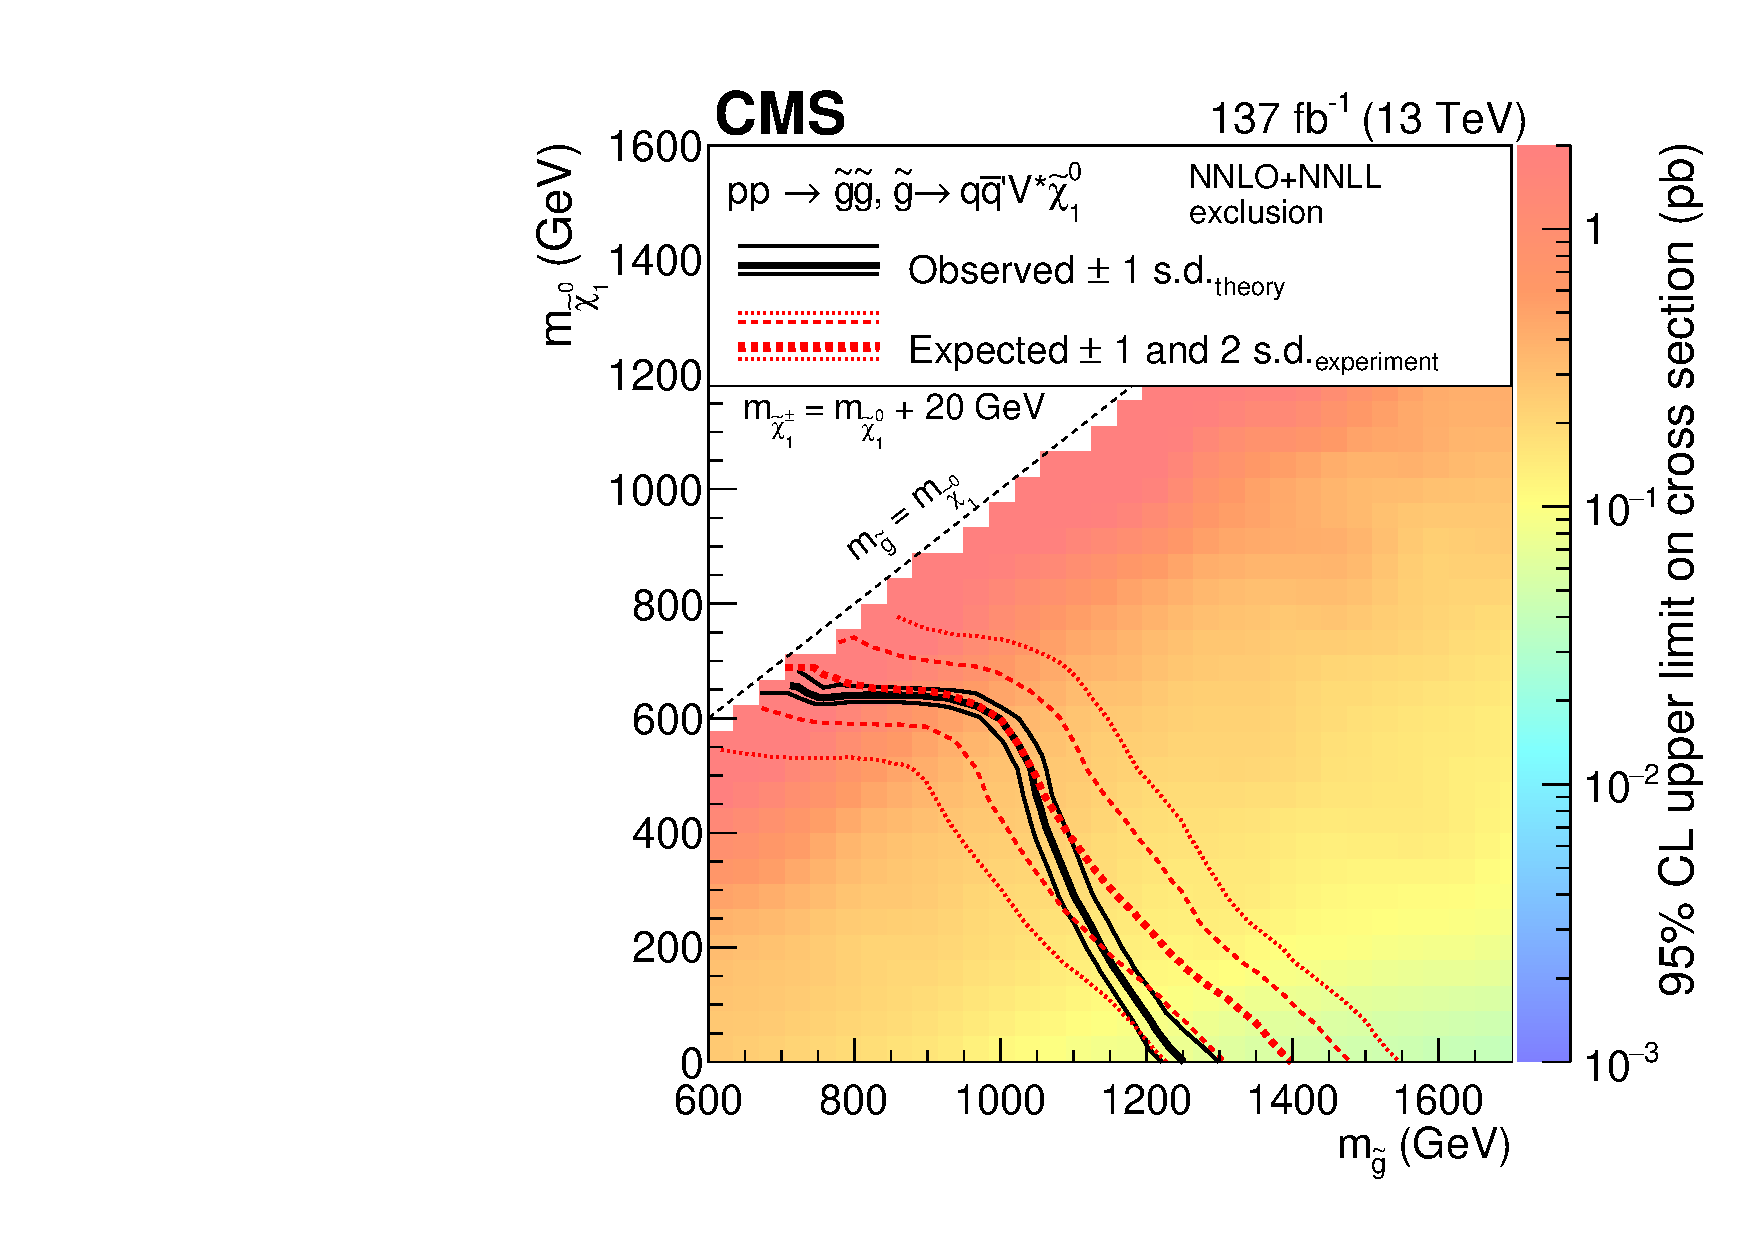
\includegraphics[width=0.45\textwidth]{figs/ssp/scan_t5qqqqvvdm20.pdf}
\caption{Exclusion regions at 95\% \CL in the plane of $m_{\lsp}$ versus $m_{\gluino}$ for the \TfqqqqWZ model
with $m_{\chiplmin}=0.5(m_{\gluino} + m_{\lsp})$~(left) and with $m_{\chiplmin} = m_{\lsp} + 20\GeV$~(right).
The notations are as in Fig.~\ref{fig:t1ttxx_scan_xsec}.  }
\label{fig:t5qqqqvv_scan_xsec}
\end{figure*}

\begin{figure*}[!hbtp]
\centering
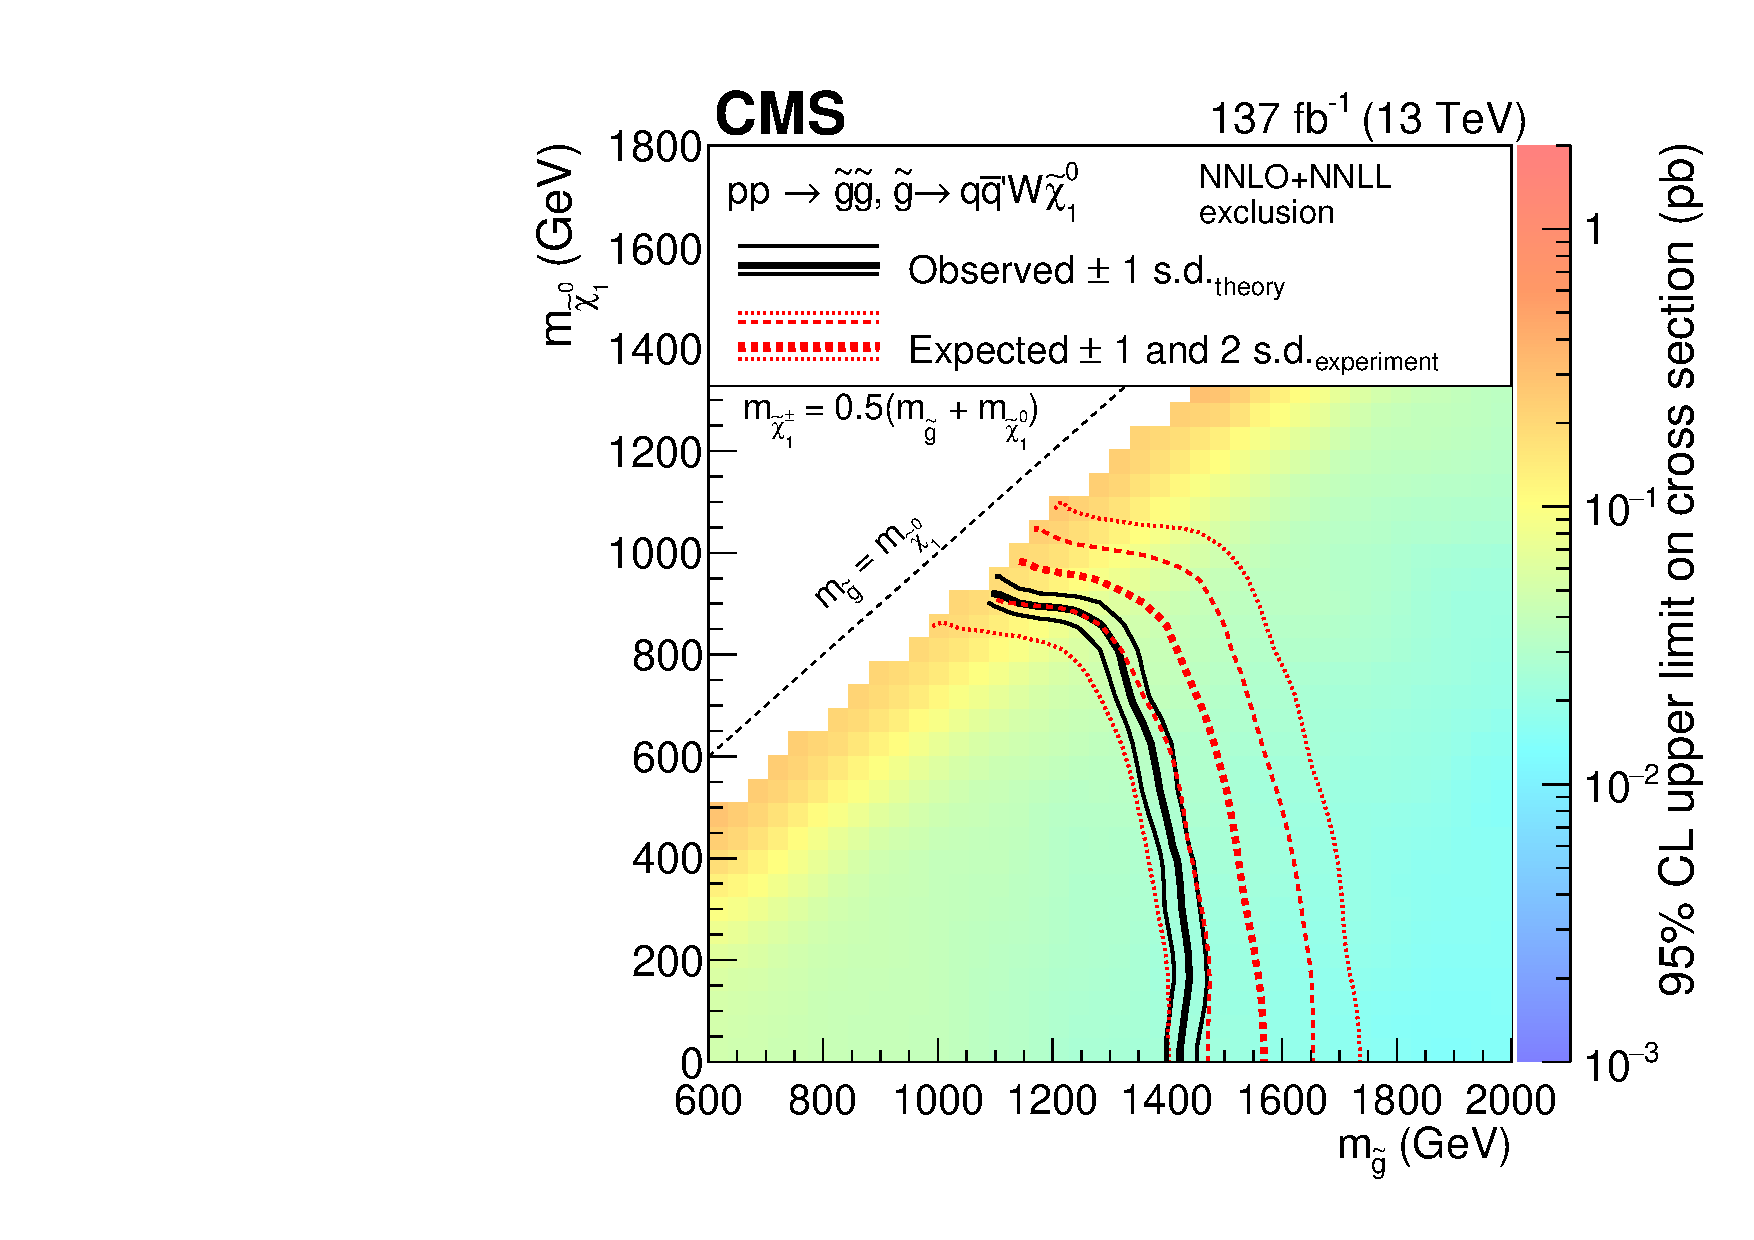
\includegraphics[width=0.45\textwidth]{figs/ssp/scan_t5qqqqww.pdf}
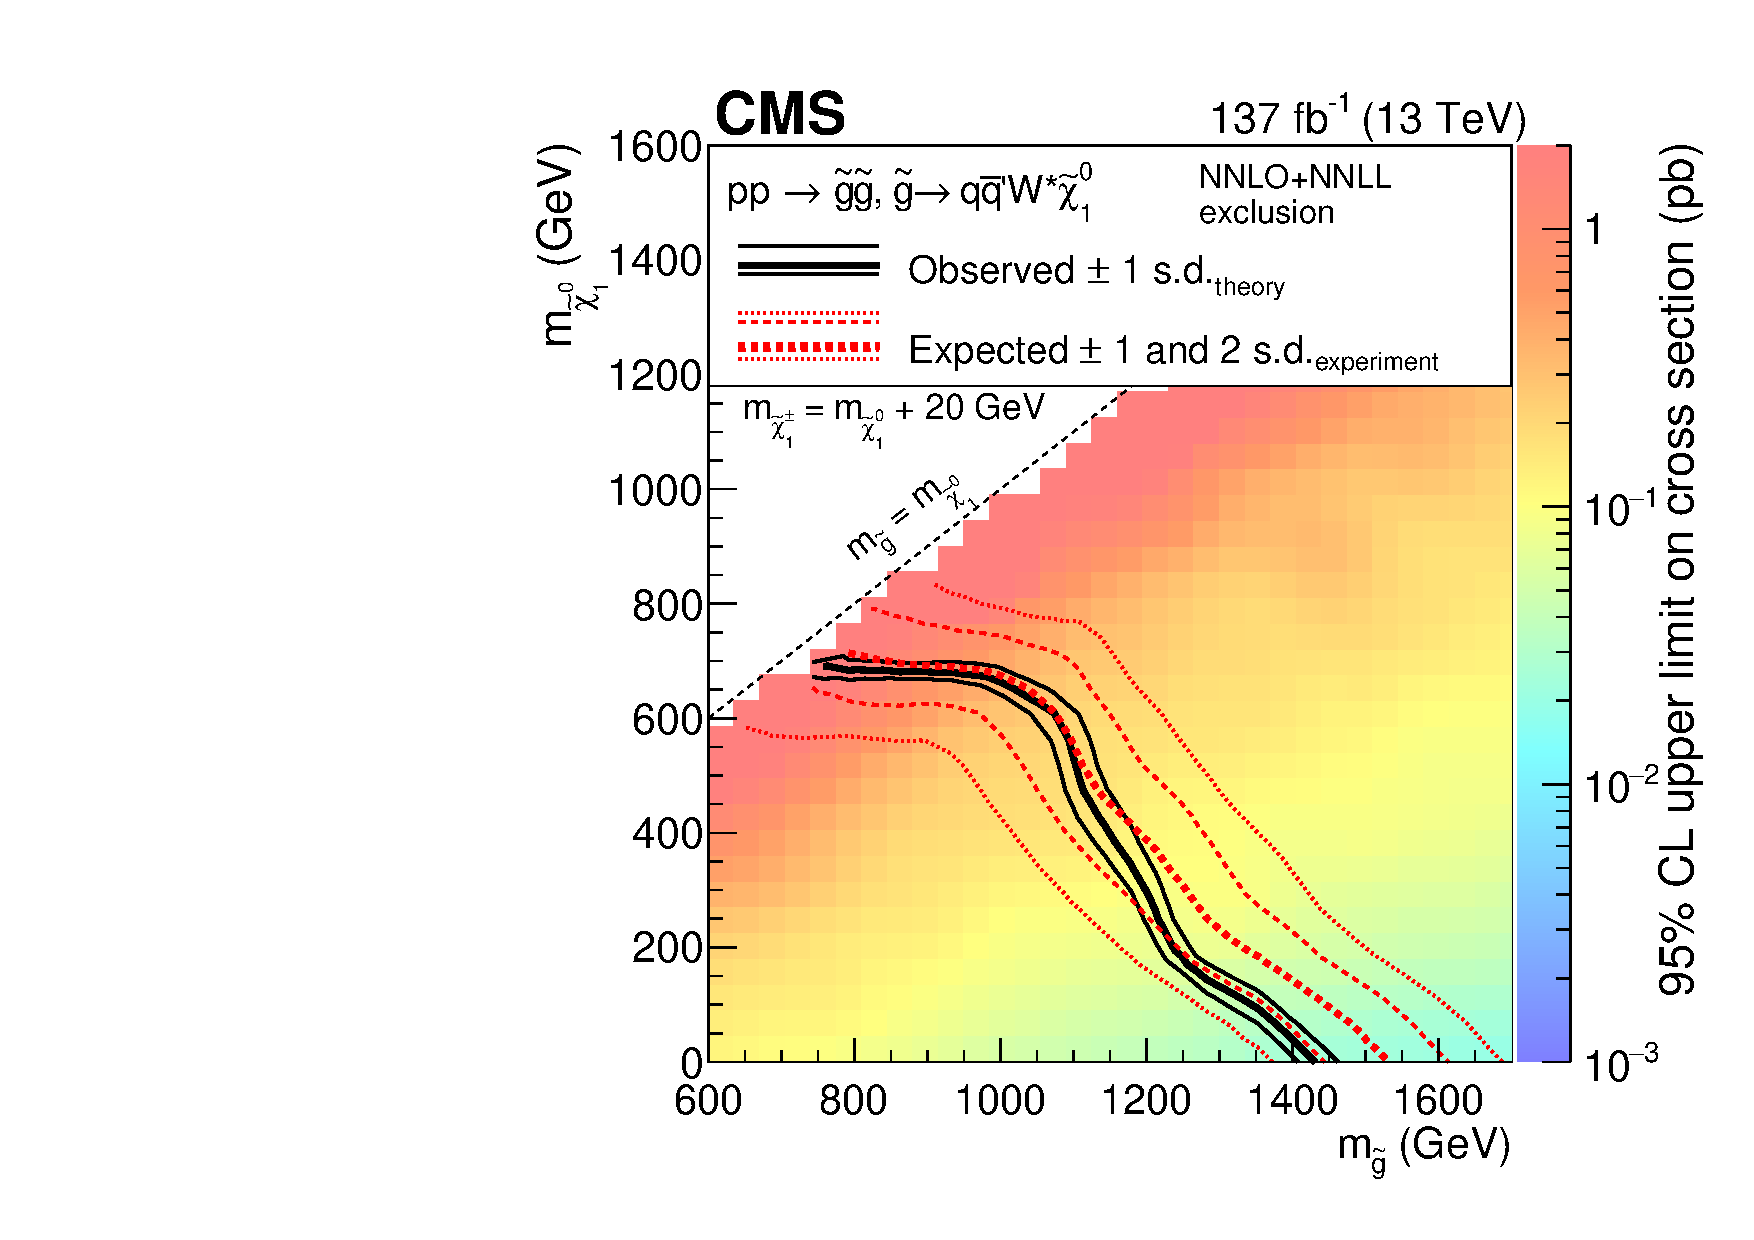
\includegraphics[width=0.45\textwidth]{figs/ssp/scan_t5qqqqwwdm20.pdf}
\caption{Exclusion regions at 95\% \CL in the plane of $m_{\lsp}$ versus $m_{\gluino}$ for the \TfqqqqWW model
with $m_{\chiplmin}=0.5(m_{\gluino} + m_{\lsp})$~(left) and with $m_{\chiplmin} = m_{\lsp} + 20\GeV$~(right).
The notations are as in Fig.~\ref{fig:t1ttxx_scan_xsec}.  }
\label{fig:t5qqqqww_scan_xsec}
\end{figure*}




\begin{figure*}[!hbtp]
\centering
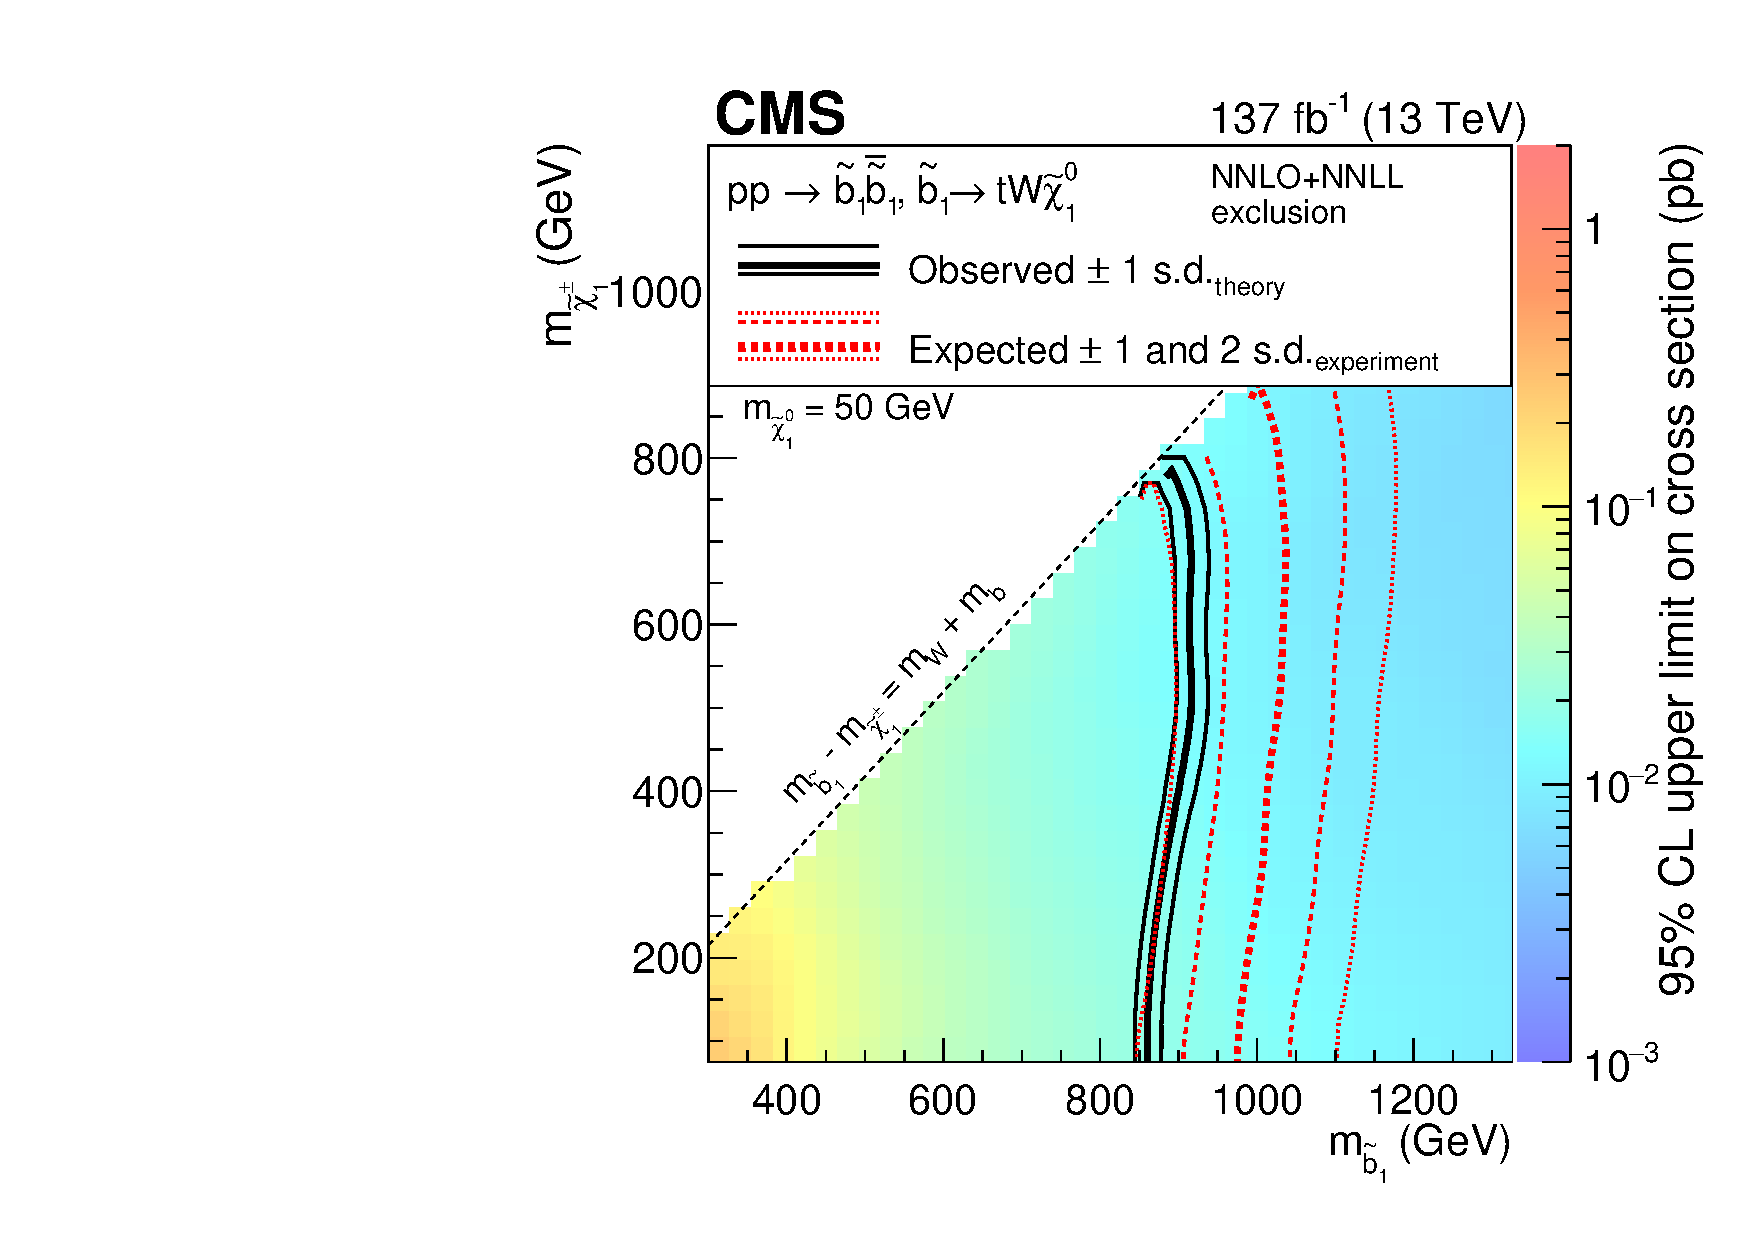
\includegraphics[width=0.60\textwidth]{figs/ssp/scan_t6ttww.pdf}\\
\caption{ Exclusion regions at 95\% \CL in the plane of $m_{\chiplmin}$ versus $m_{\sbottomone}$ for the \TsttWW model with $m_{\lsp}=50\GeV$.
    The notations are as in Fig.~\ref{fig:t1ttxx_scan_xsec}. }
\label{fig:t6ttww_scan_xsec}
\end{figure*}

\begin{figure*}[!hbtp]
\centering
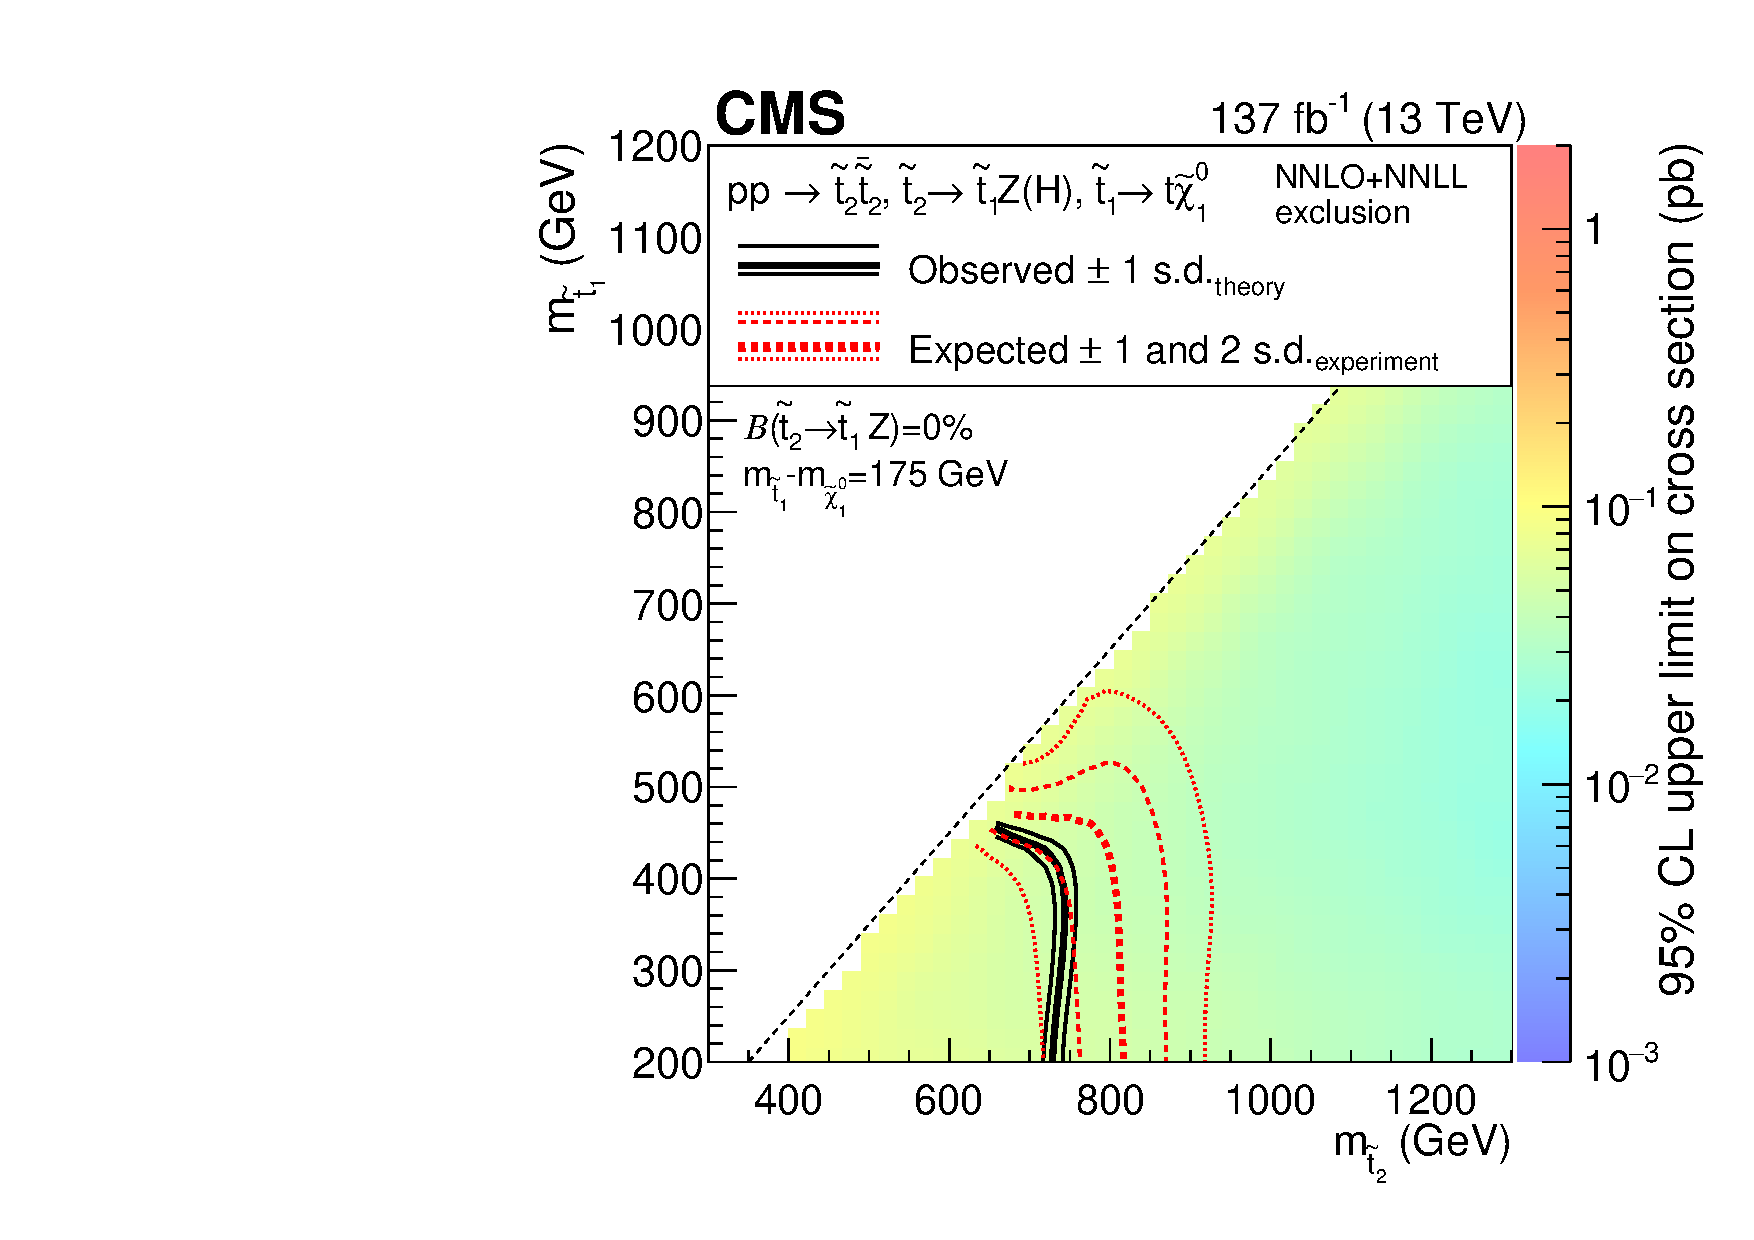
\includegraphics[width=.45\textwidth]{figs/ssp/scan_t6tthzbrh.pdf}
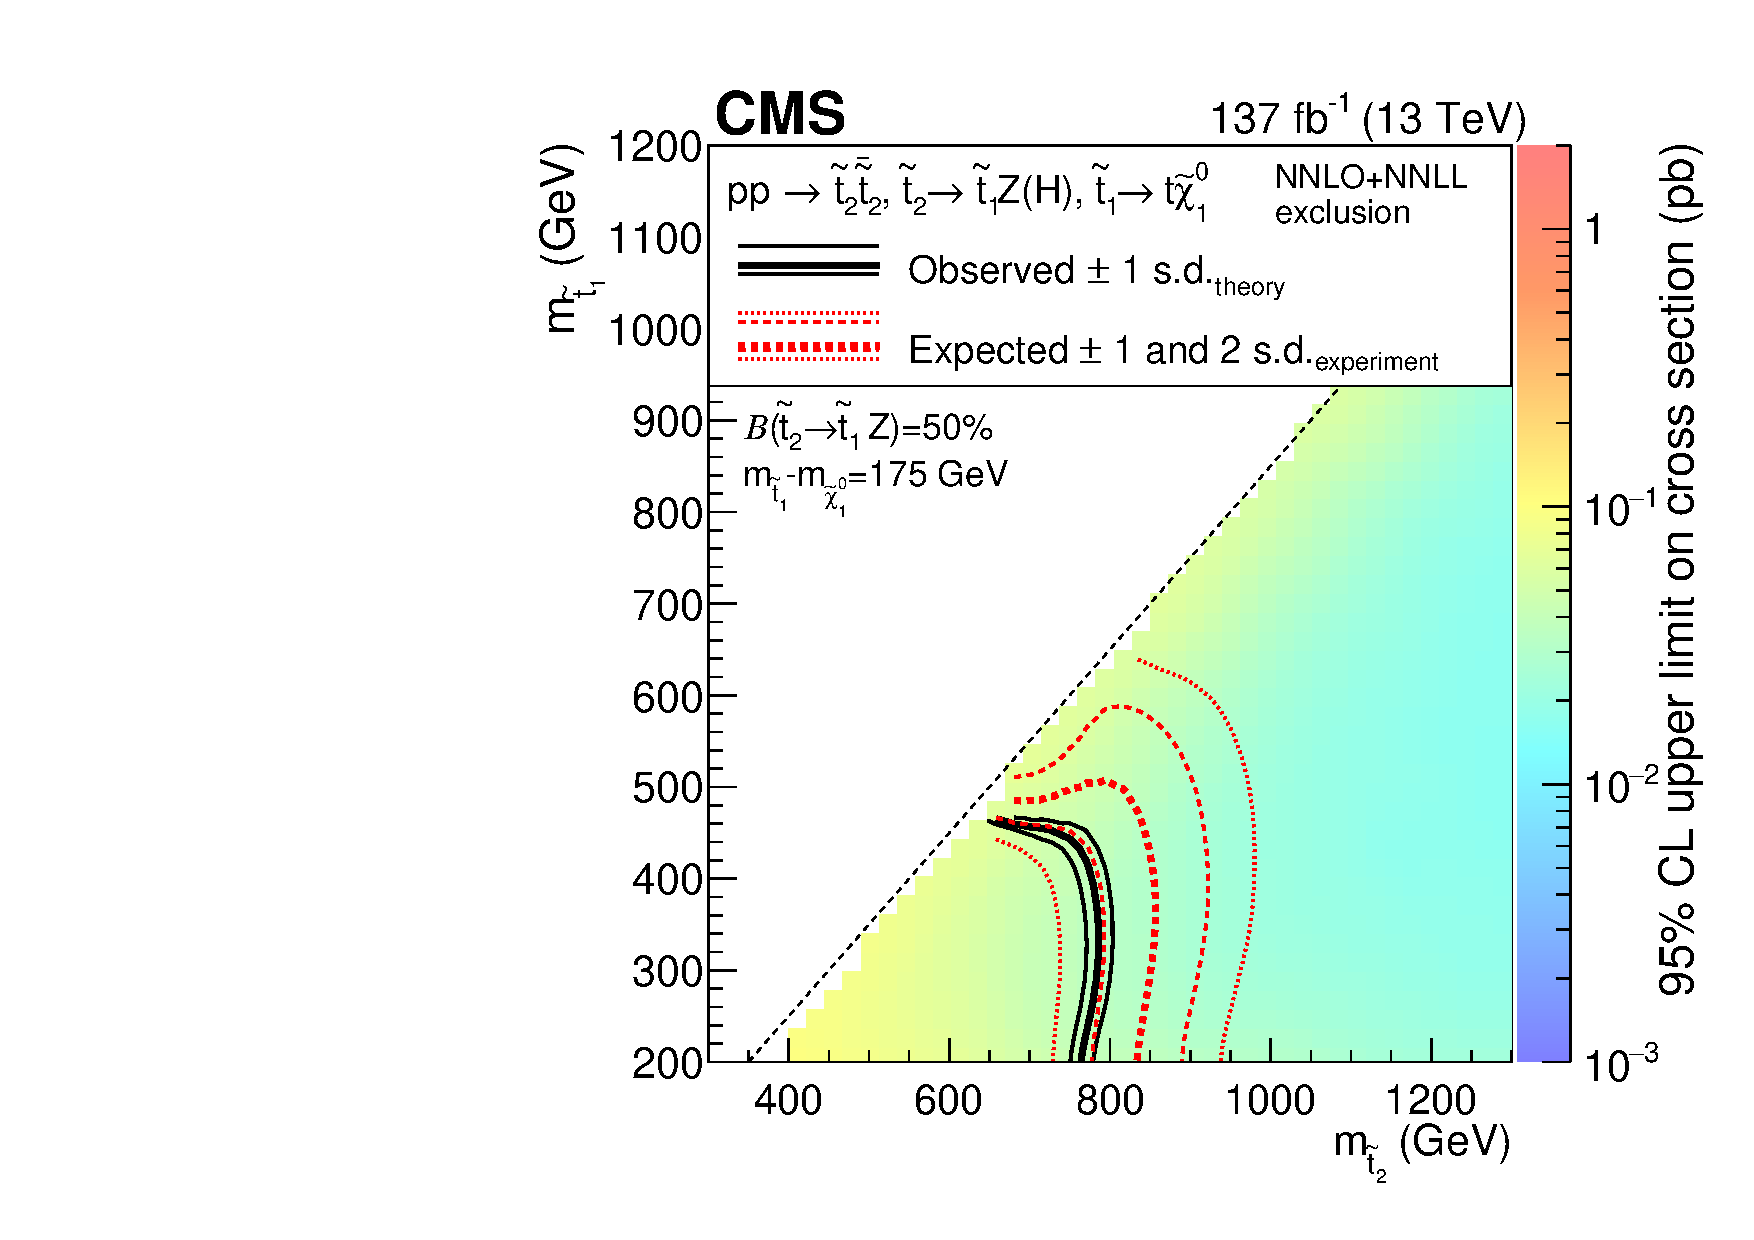
\includegraphics[width=.45\textwidth]{figs/ssp/scan_t6tthzbrb.pdf} \\
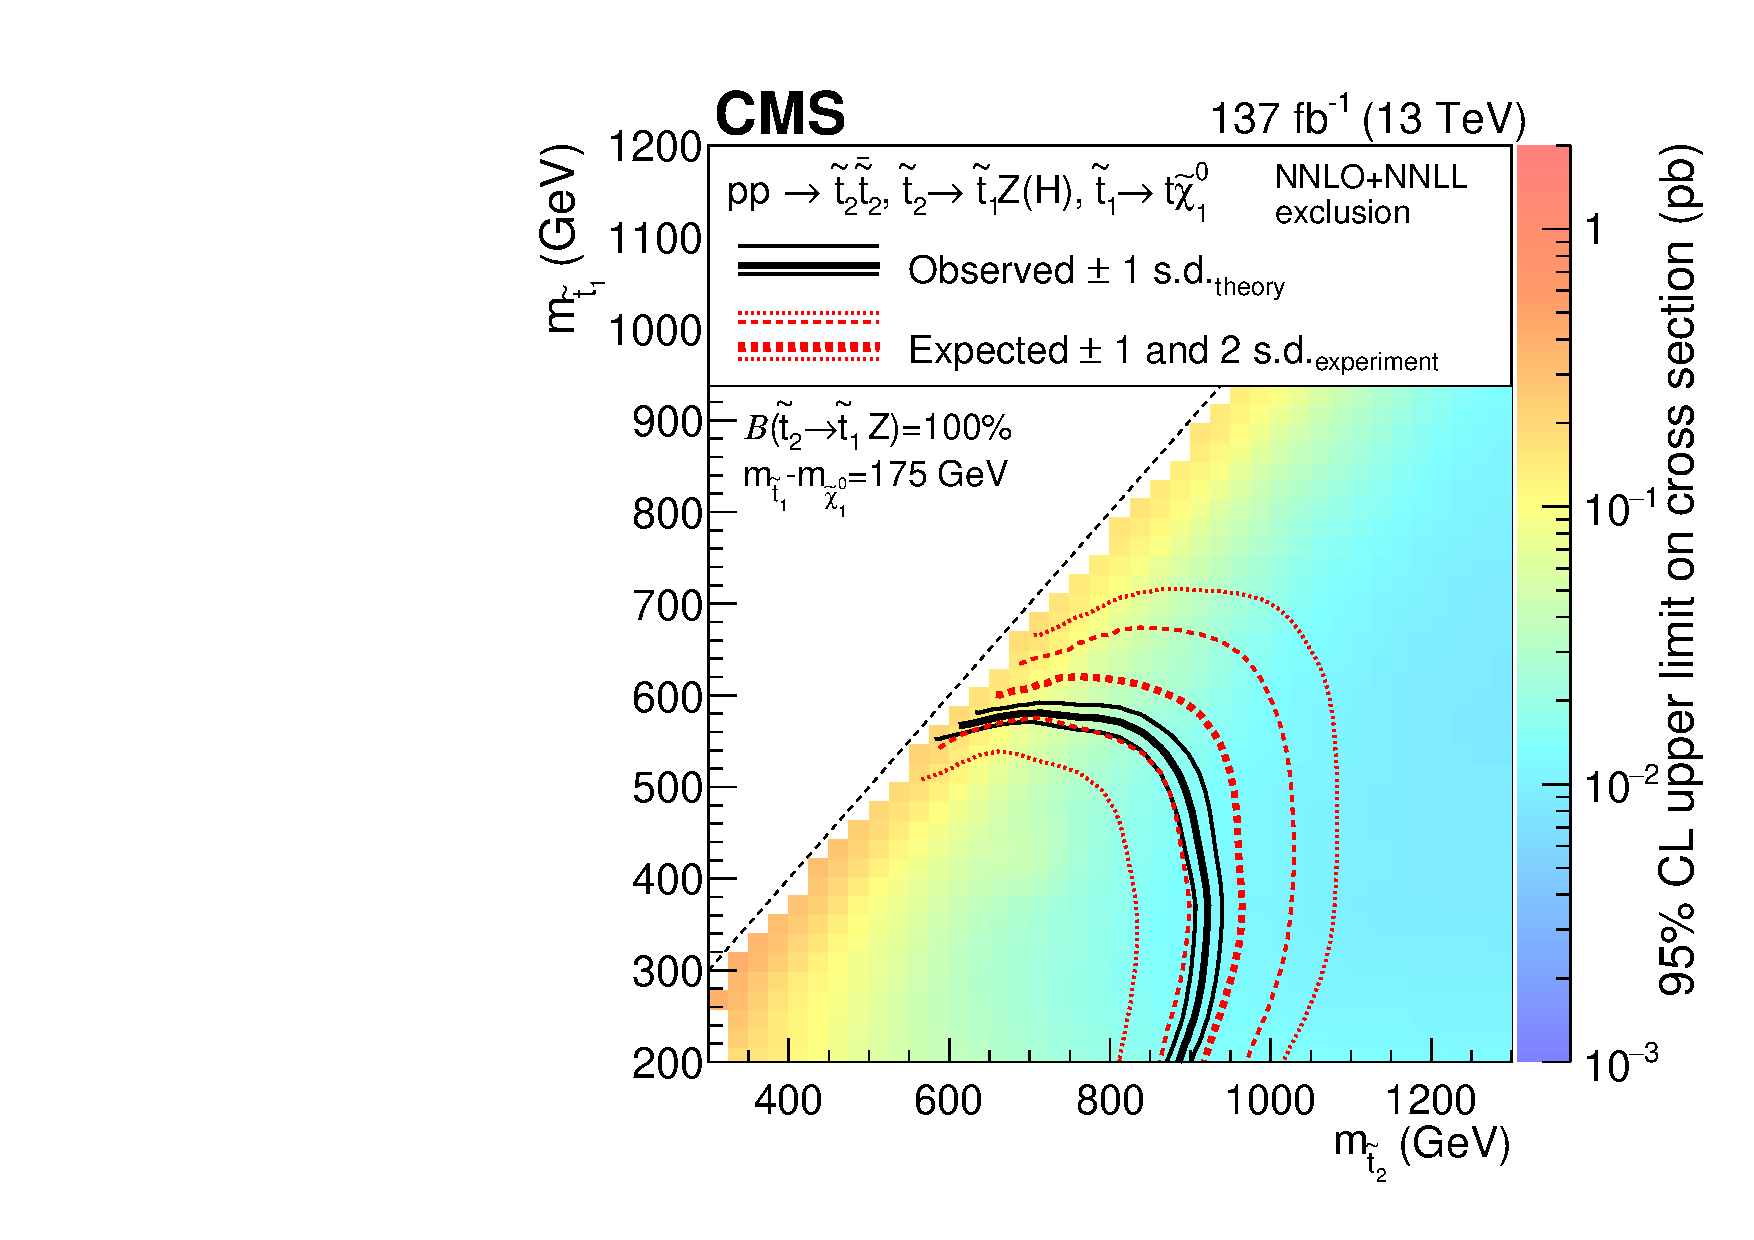
\includegraphics[width=.45\textwidth]{figs/ssp/scan_t6tthzbrz.pdf}
\\
\caption{
Exclusion regions at 95\% \CL in the plane of $m(\susytopone)$ versus
$m(\susytoptwo)$ for the \TsttHZ model with $m(\susytopone)-m(\lsp)=175\GeV$.
The three exclusions represent $\mathcal{B}(\susytoptwo\to\susytopone\PZ)$ of
0, 50, and 100\%, respectively.
The notations are as in Fig.~\ref{fig:t1ttxx_scan_xsec}.
}
\label{fig:t6tthz_scan_xsec}
\end{figure*}

\begin{figure*}[!hbtp]
\centering
    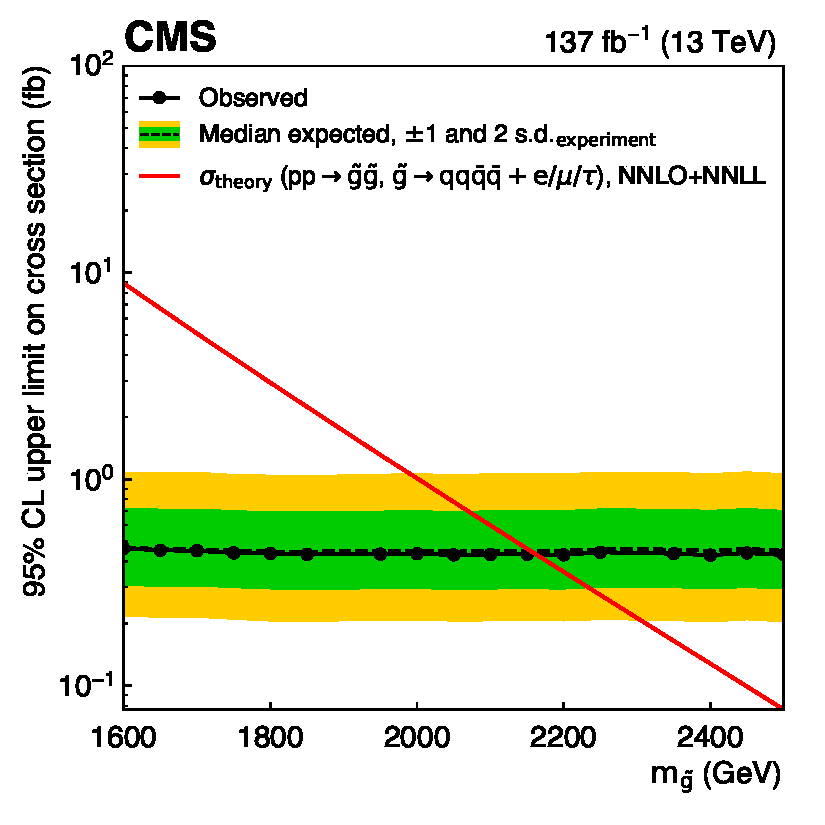
\includegraphics[width=0.45\textwidth]{figs/ssp/scan_rpv_t1qqqql.pdf}
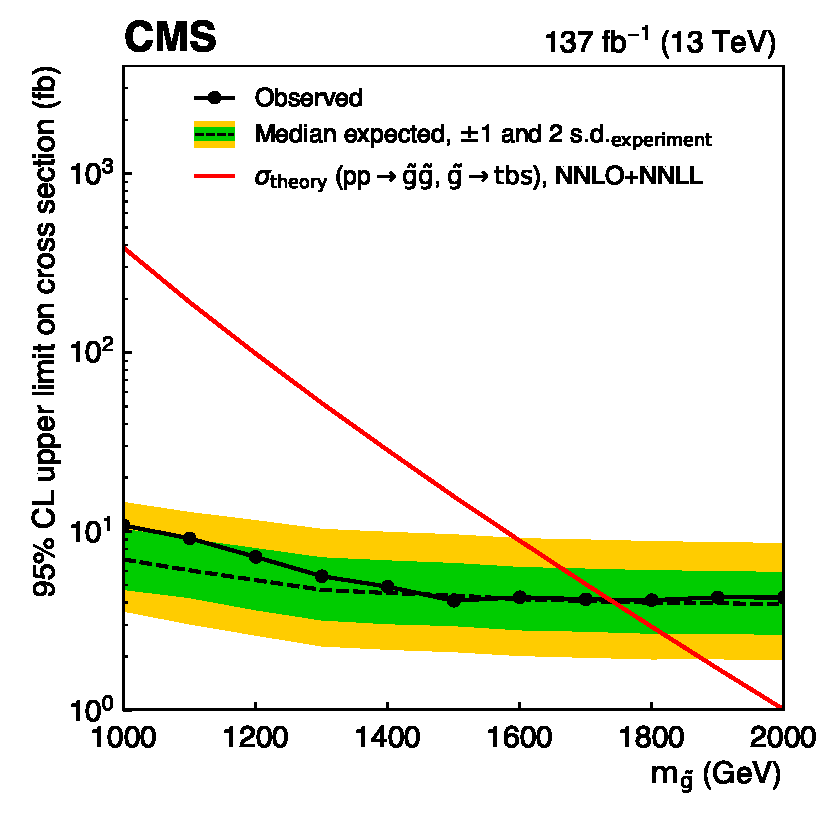
\includegraphics[width=0.45\textwidth]{figs/ssp/scan_rpv_t1tbs.pdf}\\
\caption{
          Upper limits at 95\% \CL on the cross section for RPV gluino pair production with each gluino decaying into four quarks and one lepton (\ToqqqqL, left), and
    each gluino decaying into a top, bottom, and strange quarks (\Totbs, right).
    }
\label{fig:rpvlimits}
\end{figure*}

\FloatBarrier

\subsection{Model-independent}

For the generic production of an SS lepton pair with at least two jets and
$\HT>300\GeV$, we set model-independent limits on the product of cross section, branching fraction,
detector acceptance, and reconstruction efficiency.
To do this, we select events from the HH and LM categories and calculate limits
as a function of either the minimum \ptmiss or \HT requirements starting at 
300 and 1400\GeV, respectively. Because there is an overlap between the two conditions,
events that are selected for the limits as a function of \HT must also have 
$\ptmiss<300\GeV$. Both sets of limits are shown in Fig.~\ref{fig:milimits}.

In order to assist with future reinterpretations of the inclusive same-sign
search results shown here, we calculated the expected and observed yields for
a set of inclusive SRs, shown in Table~\ref{tab:inclusive_aggregate}. The
last column in the table indicates the upper limit at 95\% \CL on the number
of BSM events in each SR. The SRs are defiend to have on the order of 5 to 10
expected background events, and we focus on events with large \HT, \ptmiss,
\Nbjets, and/or \Njets. No uncertainty in the signal acceptance is assumed in
calculating the limits in the table.




\begin{figure*}[!hbtp]
\centering
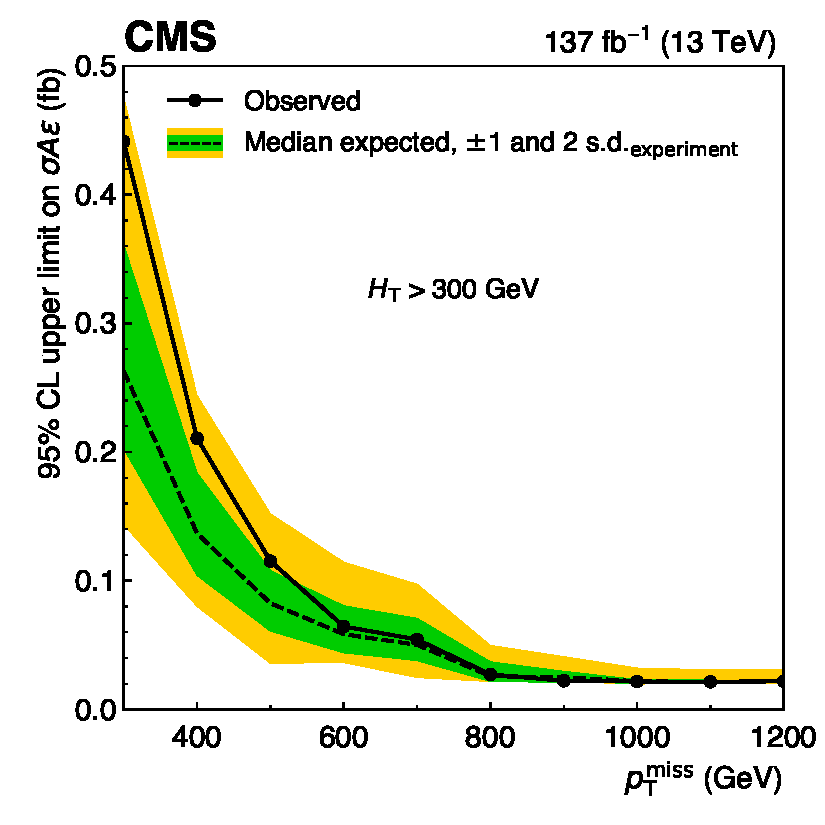
\includegraphics[width=0.45\textwidth]{figs/ssp/scan_milimits_met.pdf}
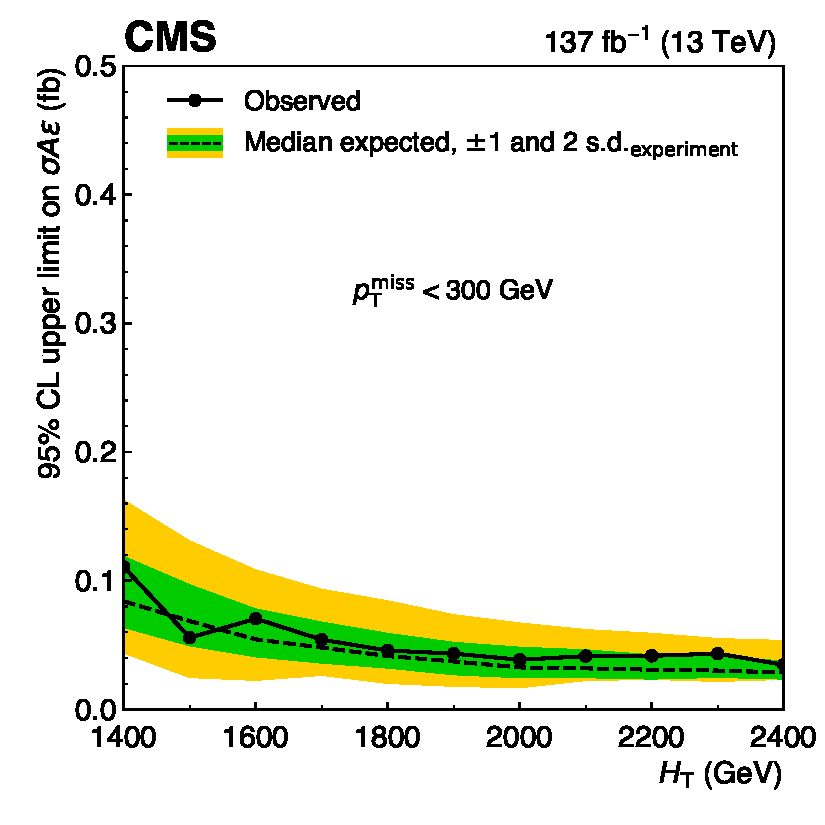
\includegraphics[width=0.45\textwidth]{figs/ssp/scan_milimits_ht.pdf}
\caption{Upper limits at 95\% \CL on the product of cross section, detector acceptance, and selection efficiency, $\sigma \! \mathcal{A} \epsilon$,
for the production of an SS lepton pair with at least two jets, as a function of the minimum \ptmiss threshold, when $\HT>300\GeV$ (left), or the minimum \HT threshold, when $\ptmiss<300\GeV$ (right).
    }
\label{fig:milimits}
\end{figure*}

\begin{table}[!h]
\centering
\label{tab:inclusive_aggregate}
{\renewcommand{\arraystretch}{1.3}
\resizebox{0.99\textwidth}{!}{
  \begin{tabular}{c|cccccc|ccc}
  \hline
         SR     & Category              & \Njets   & \Nbjets  & \HT (\GeV)  & \ptmiss (\GeV) & \mtmin (\GeV) & SM expected       & Obs.  &  $N_\text{BSM}^\text{max} (95\%\ \CL)$ \\
         \hline
        ISR1  & \multirow{11}{*}{HH} & $\geq$2  & 0        & $\geq$1000  & $\geq$250  & \NA        & $12.7 \pm 7.4$ & 16 & 12.32  \\
        ISR2  &                      & $\geq$2  & $\geq$2  & $\geq$1100  & \NA        & \NA        & $11.0 \pm 3.8$ & 14 & 11.33  \\
        ISR3  &                      & $\geq$2  & 0        & \NA         & $\geq$500  & \NA        & $10.4 \pm 9.7$ & 13 & 11.26  \\
        ISR4  &                      & $\geq$2  & $\geq$2  & \NA         & $\geq$300  & \NA        & $11.4 \pm 3.8$ & 17 & 14.22  \\
        ISR5  &                      & $\geq$2  & 0        & \NA         & $\geq$250  & $\geq$120  & $6.6 \pm 5.7$  & 10 & 10.77  \\
        ISR6  &                      & $\geq$2  & $\geq$2  & \NA         & $\geq$200  & $\geq$120  & $6.3 \pm 1.3$  & 8  & 8.22   \\
        ISR7  &                      & $\geq$8  & \NA      & \NA         & \NA        & \NA        & $7.0 \pm 2.8$  & 12 & 12.17  \\
        ISR8  &                      & $\geq$6  & \NA      & \NA         & \NA        & $\geq$120  & $6.2 \pm 1.4$  & 10 & 10.45  \\
        ISR9  &                      & $\geq$2  & $\geq$3  & $\geq$800   & \NA        & \NA        & $7.8 \pm 3.5$  & 8  & 7.53   \\
        \hline
        ISR10 & \multirow{4}{*}{LL}  & $\geq$2  & \NA      & $\geq$700   & \NA        & \NA        & $10.4 \pm 9.0$ & 12 & 10.37  \\
        ISR11 &                      & $\geq$2  & \NA      & \NA         & $\geq$200  & \NA        & $12.1 \pm 5.6$ & 13 & 9.94   \\
        ISR12 &                      & $\geq$6  & \NA      & \NA         & \NA        & \NA        & $7.1 \pm 4.3$   & 7  & 7.10   \\
        ISR13 &                      & $\geq$2  & $\geq$3  & \NA         & \NA        & \NA        & $1.61 \pm 0.39$ & 3  & 5.70   \\
        \hline
        ISR14 & \multirow{2}{*}{LM}  & $\geq$2  & 0        & $\geq$1200  & $<$50      & \NA        & $3.6 \pm 3.6$   & 3  & 5.10   \\
        ISR15 &                      & $\geq$2  & $\geq$2  & $\geq$1000  & $<$50      & \NA        & $2.34 \pm 0.51$ & 4  & 6.41   \\
        \hline
        ISR16 & \multirow{2}{*}{ML}  & $\geq$2  & 0        & $\geq$1000  & $\geq$300  & \NA        & $5.6 \pm 1.6$   & 7  & 7.78   \\
        ISR17 &                      & $\geq$2  & $\geq$2  & $\geq$1000  & \NA        & \NA        & $5.7 \pm 1.9$   & 7  & 7.62   \\ \hline
\end{tabular}}
}
\caption{
    Inclusive SR definitions, expected background yields and uncertainties, and observed yields, as well as the observed 95\% \CL upper limits on the number of BSM events contributing to each region.
    % No uncertainty in the signal acceptance is assumed in calculating these limits. A dash (\NA) indicates that a particular selection is not required.
    A dash (\NA) indicates that a particular selection is not required.
}
\end{table}

\FloatBarrier

\section{\smft results}
\label{sec:ftresults}

Distributions of the main kinematic variables in the \smft analysis (\Njets, \Nbjets, \HT, and
\ptmiss) for events passing the baseline selections are shown in Fig.~\ref{fig:kinemsr} and compared
to the SM background predictions. 
The \Njets and \Nbjets distributions for
the \ttW and \ttZ control regions, CRW and CRZ, are shown in Fig.~\ref{fig:kinemcr}. 
In both figures, the expected SM \tttt
signal is normalized to its predicted cross section.
Again, fortunately (or unfortunately), {\it the SM predictions are statistically consistent with the observations.}

\begin{figure*}[!hbt]
\centering
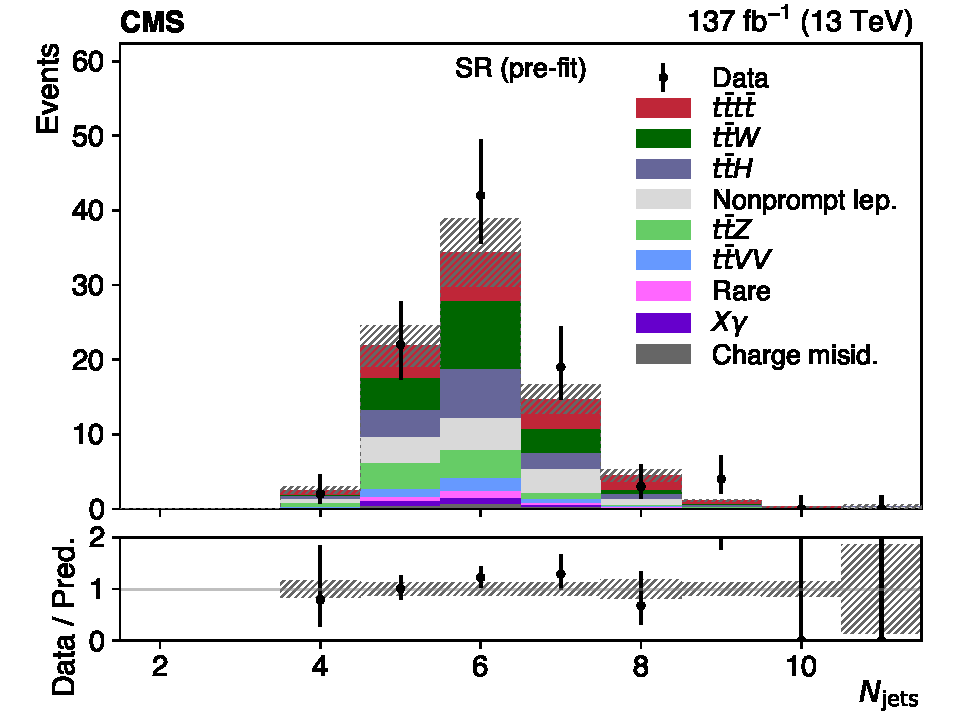
\includegraphics[width=.49\textwidth]{figs/ftp/sr_njets_prefit.pdf}
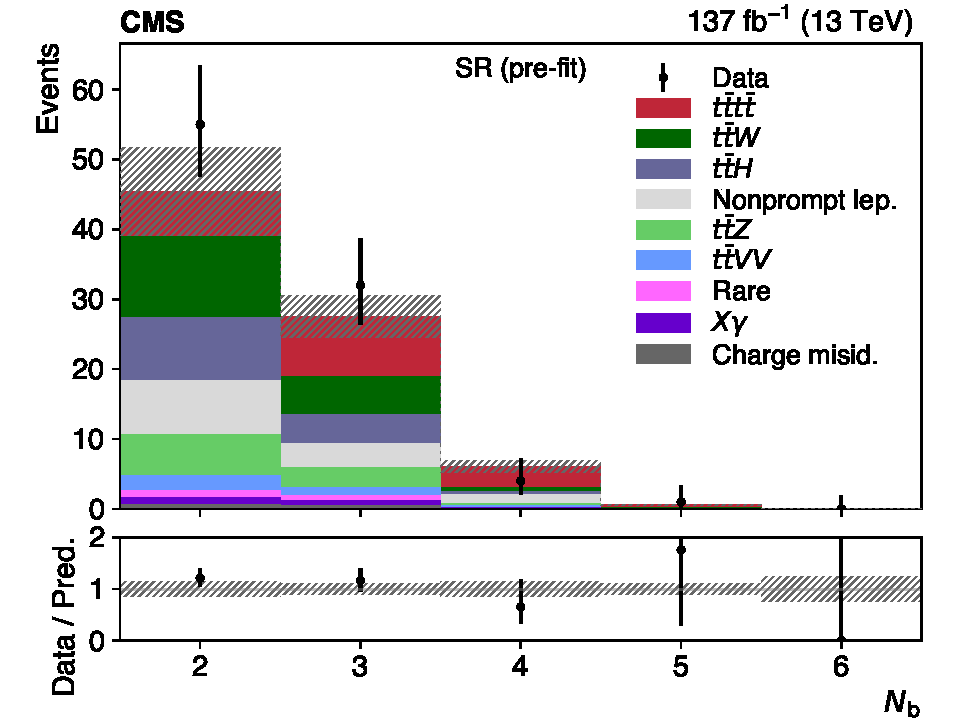
\includegraphics[width=.49\textwidth]{figs/ftp/sr_nbtags_prefit.pdf}
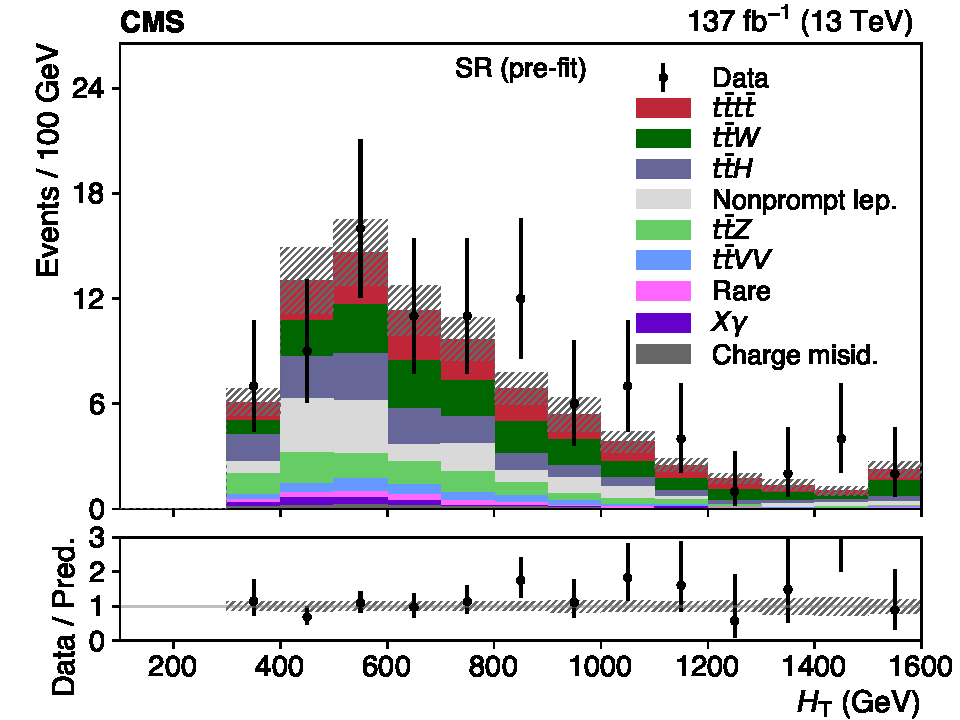
\includegraphics[width=.49\textwidth]{figs/ftp/sr_ht_prefit.pdf}
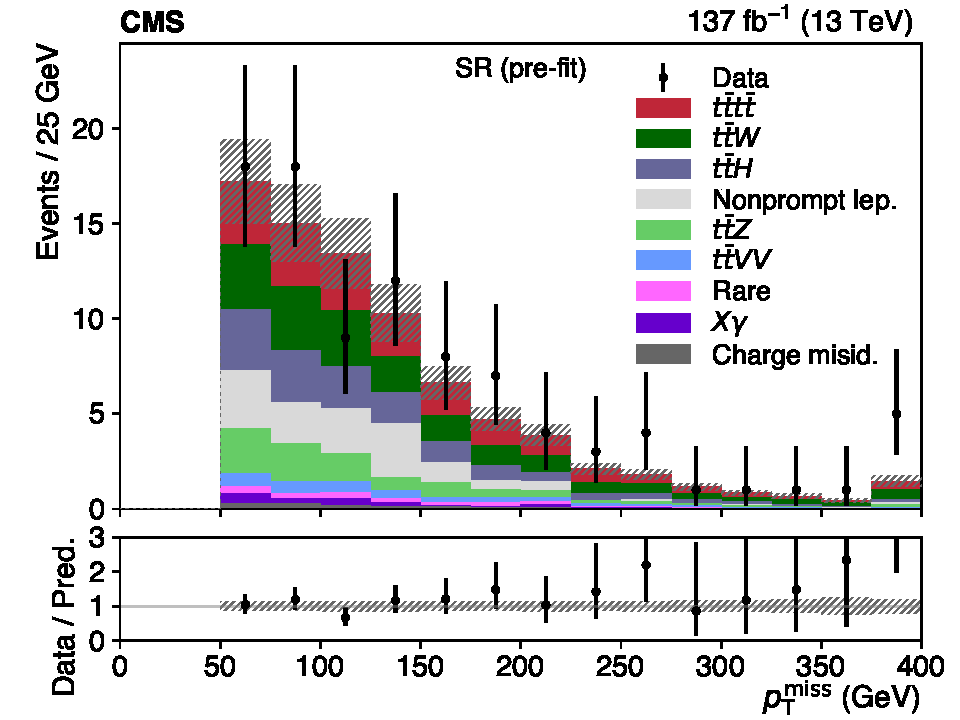
\includegraphics[width=.49\textwidth]{figs/ftp/sr_met_prefit.pdf}
\caption{ Distributions of \Njets (upper left), \Nbjets (upper right), \HT (lower left), and \ptmiss (lower right) in the summed SRs (1--14), before fitting to data,
where the last bins include the overflows. The hatched areas represent the total uncertainties in the SM signal and background predictions.
 The lower panels show the ratios of the observed event yield to the total prediction of
    signal plus background.
    }
\label{fig:kinemsr}
\end{figure*}

\begin{figure*}[!hbt]
\centering
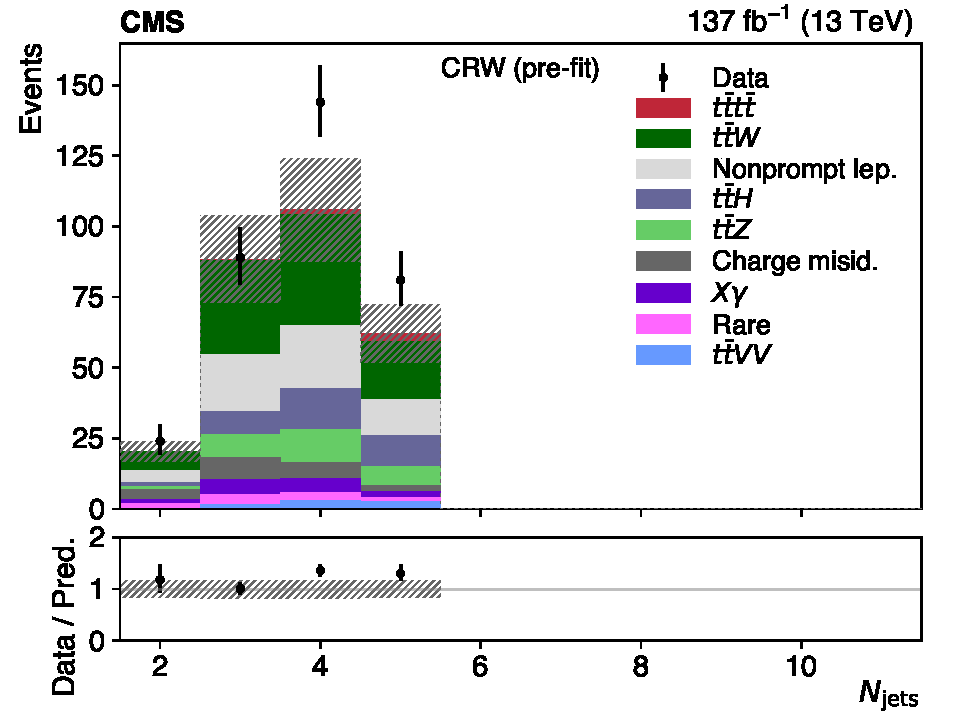
\includegraphics[width=.49\textwidth]{figs/ftp/ttwcr_njets_prefit.pdf}
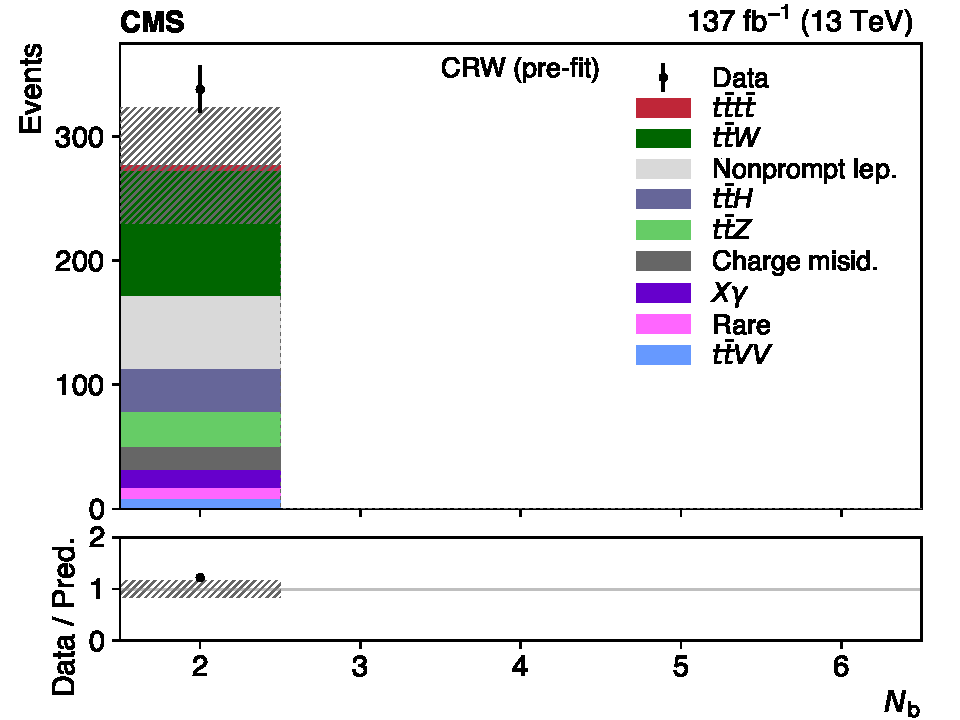
\includegraphics[width=.49\textwidth]{figs/ftp/ttwcr_nbtags_prefit.pdf}
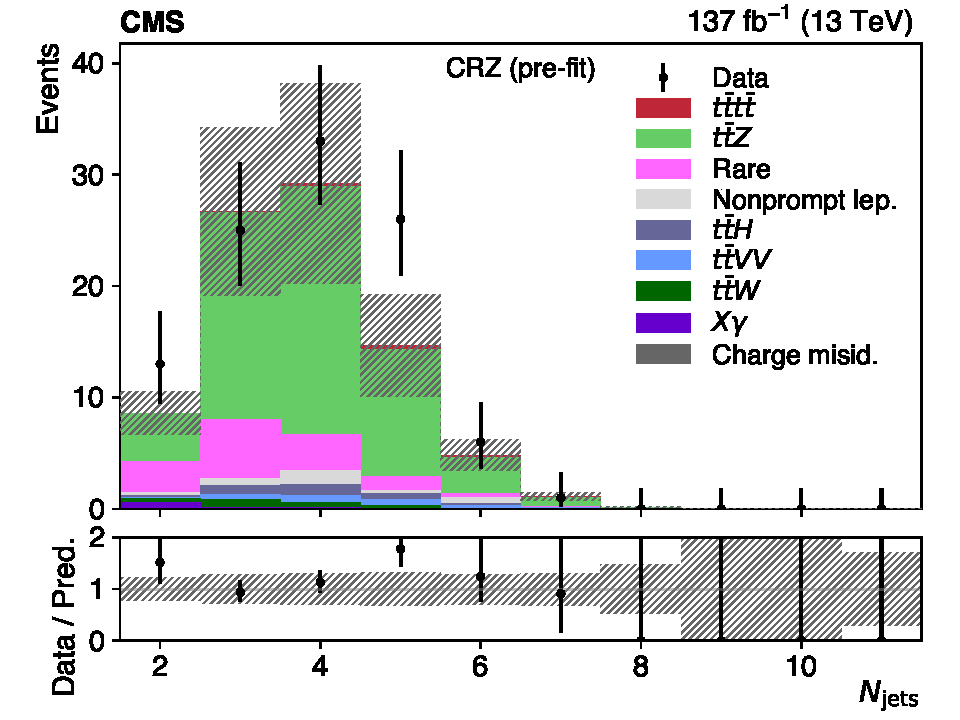
\includegraphics[width=.49\textwidth]{figs/ftp/ttzcr_njets_prefit.pdf}
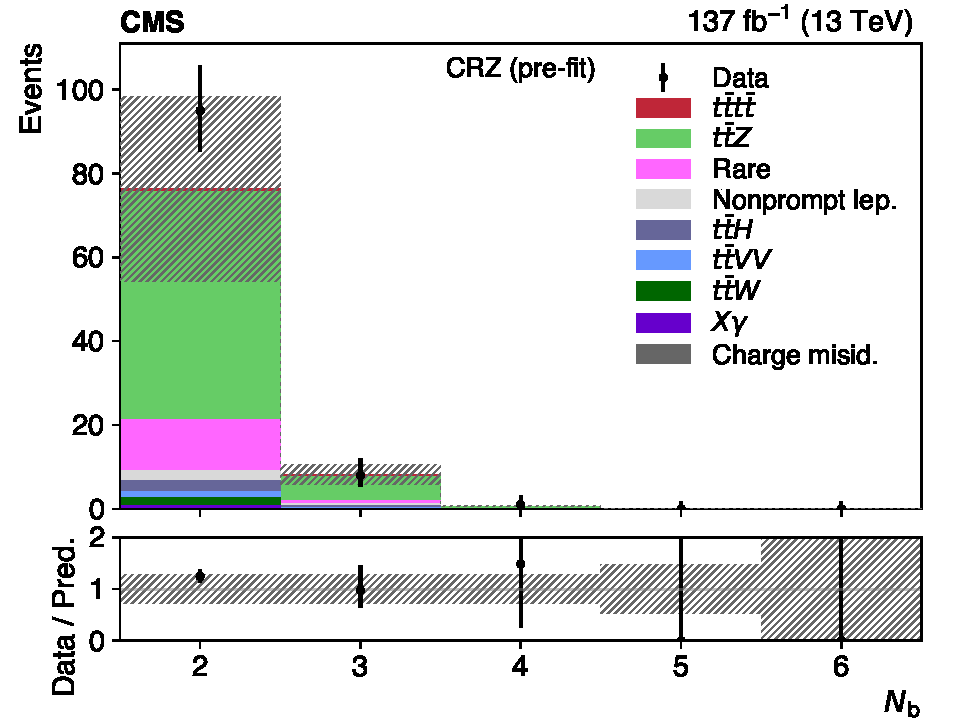
\includegraphics[width=.49\textwidth]{figs/ftp/ttzcr_nbtags_prefit.pdf}
    \caption{Distributions of \Njets (left) and \Nbjets (right) in the \ttW (upper) and \ttZ (lower) CRs, before fitting to data.
The hatched areas represent the  uncertainties in the SM signal and background predictions.
 The lower panels show the ratios of the observed event yield to the total prediction of
    signal plus background.
    }
\label{fig:kinemcr}
\end{figure*}

The yields from the SRs, CRZ, and CRW (for the cut-based analysis only),
incorporating experimental and theoretical uncertainties as ``nuisance''
parameters, are used to construct a binned likelihood function.
The measured cross
section for \tttt and the statistical significance of the observation relative to the
background-only hypothesis are obtained from a profile maximum-likelihood
fit, in which the parameter of interest is \xsectttt and all nuisance
parameters are profiled, following the procedures described in
Refs.~\cite{STAT:ATLPHYSPUB2011011,STAT:PDG}. 
An upper limit at 95\%
confidence level (\CL) is set on \xsectttt using the 
\CLs criterion~\cite{STAT:Junk1999kv,STAT:Read2002hq}, 
and asymptotic approximation~\cite{STAT:Cowan2010js}. 
Alternatively, by considering the SM, including the \tttt process with the SM
cross section and uncertainty~\cite{THEORY:Frederix2017wme}, as the null
hypothesis, the fit provides cross section upper limits on BSM processes with
new scalar and pseudoscalar particles, which will come into play when
considering the interpretations in the upcoming sections.

While the values of most nuisance parameters are unchanged by the
fit, the ones significantly affected include those corresponding to the
\ttW and \ttZ normalizations, which are both scaled by $1.3\pm0.2$ by the
fit. This is in agreement with recent ATLAS and CMS measurements of these
processes~\cite{ATLAS:Aaboud2019njj, CMS:Sirunyan2017uzs, CMS:2019too}, which
measures an underprediction of \ttW and \ttZ processes at NLO when compared to
data, by approximately 20-30\%. The
post-fit predicted yields are compared to
data in Fig.~\ref{fig:srcr} for the cut-based and BDT 
analyses, where the fitted \tttt signal contribution is stacked on to the
background predictions. The corresponding yields are shown in
Tables~\ref{tab:srcryields} and \ref{tab:srdiscyields} for the cut-based and
BDT analysis, respectively.

The \tttt cross section and the 68\% \CL interval is measured to be
$9.4^{+6.2}_{-5.6}~\unit{fb}$ in the cut-based analysis, and
$12.6^{+5.8}_{-5.2}~\unit{fb}$ in the BDT analysis. Relative to the
background-only hypothesis, the observed and expected significances are 1.7
and 2.5 standard deviations, respectively, for the cut-based analysis, and
2.6 and 2.7 standard deviations for the BDT analysis. The observed 95\% \CL
upper limits on the cross section are $20.0~\unit{fb}$ in the cut-based and
$22.5~\unit{fb}$ in the BDT analyses. The corresponding expected upper limits
on the \tttt cross section, assuming no SM \tttt contribution to the data,
are $9.4^{+4.3}_{-2.9}~\unit{fb}$ (cut-based) and $8.5^{+3.9}_{-2.6}~\unit{fb}$
(BDT), a significant improvement relative to the value of
$20.8^{+11.2}_{-6.9}~\unit{fb}$ of Ref.~\cite{CMS:myTOP2016}. Because it 
provides a higher expected measurement precision, we consider the BDT
analysis as the primary result with which to perform further interpretations.

\begin{figure}[!hbtp]
\centering
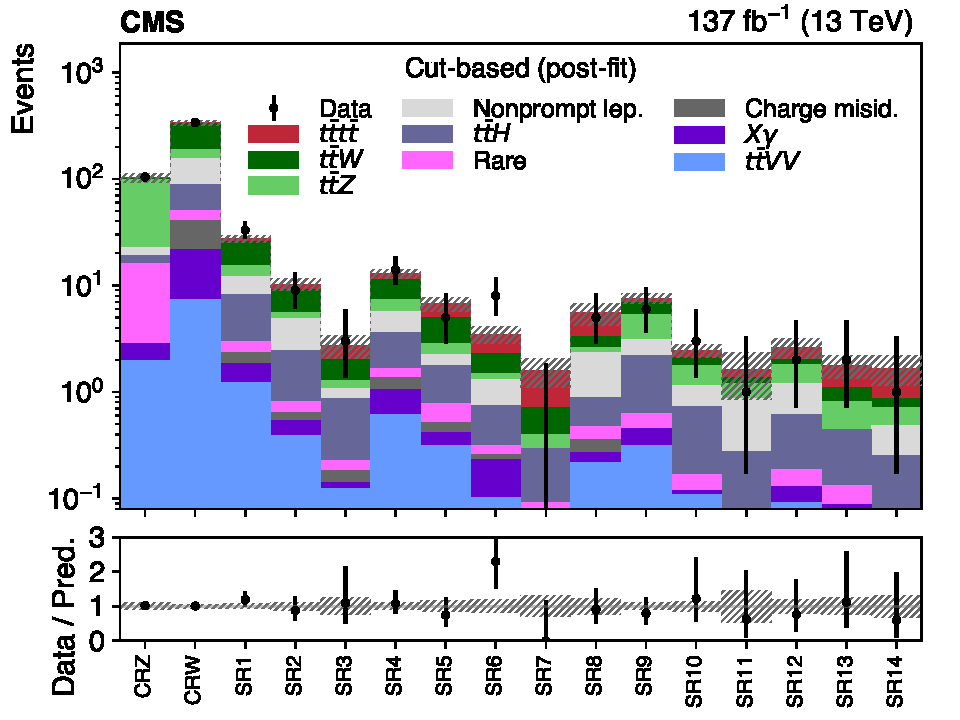
\includegraphics[width=0.8\textwidth]{figs/ftp/SRCR_postfit.pdf} \\
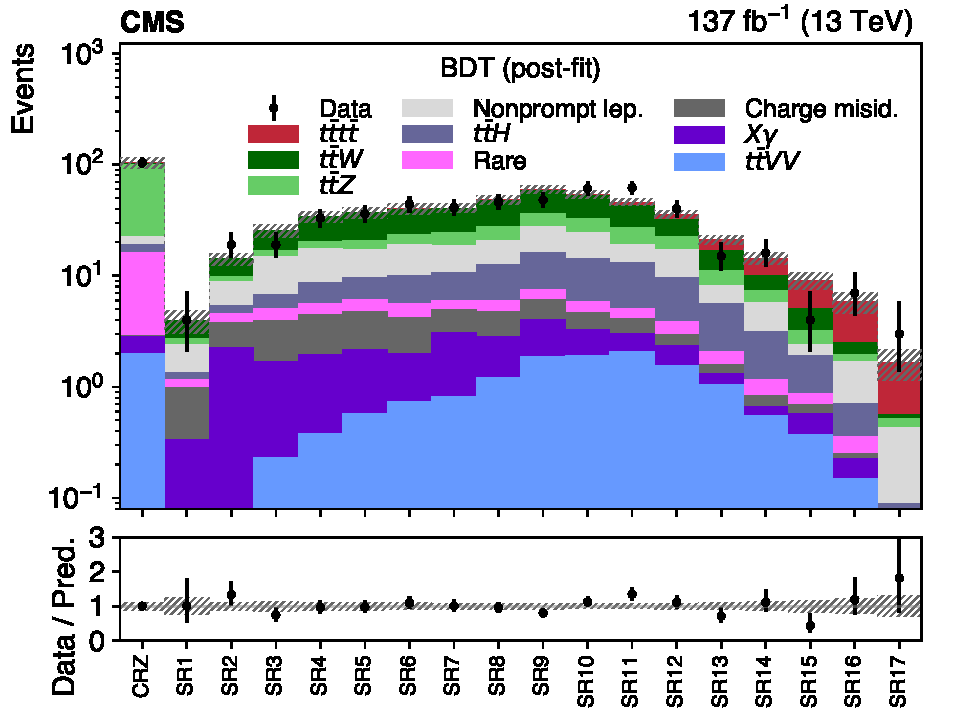
\includegraphics[width=0.8\textwidth]{figs/ftp/SRDISC_postfit.pdf}
\caption{ Observed yields in the control and signal regions for the cut-based (upper) and BDT (lower) analyses,
compared to the post-fit predictions for signal and background processes.
The hatched areas represent the total post-fit uncertainties in the signal and background predictions.
The lower panels show the ratios of the observed event yield to the total prediction of
    signal plus background.
    }
\label{fig:srcr}
\end{figure}


\begin{table}[htb!]
\centering
\label{tab:srcryields}
{\renewcommand{\arraystretch}{1.2}
    \begin{tabular}{ccccc}
        & SM background  & $\tttt$   & Total   & Observed \\
            \hline
CRZ  & $101\pm10\ \ $   & $0.83\pm0.49$ & $102\pm10\ \ $   & 104 \\
CRW  & $331\pm19\ \ $   & $3.9\pm2.3$   & $335\pm18\ \ $   & 338 \\
SR1  & $25.6\pm2.1\ \ $ & $2.0\pm1.2$   & $27.6\pm2.1\ \ $ & 33 \\
SR2  & $9.1\pm1.3$      & $1.13\pm0.65$ & $10.3\pm1.3\ \ $ & 9 \\
SR3  & $2.01\pm0.58$    & $0.73\pm0.42$ & $2.74\pm0.67$    & 3 \\
SR4  & $11.3\pm1.3\ \ $ & $1.58\pm0.90$ & $12.9\pm1.3\ \ $ & 14 \\
SR5  & $5.03\pm0.77$    & $1.68\pm0.95$ & $6.7\pm1.1$      & 5 \\
SR6  & $2.29\pm0.40$    & $1.20\pm0.67$ & $3.48\pm0.66$    & 8 \\
SR7  & $0.71\pm0.20$    & $0.88\pm0.48$ & $1.59\pm0.49$    & 0 \\
SR8  & $3.31\pm0.95$    & $2.2\pm1.3$   & $5.5\pm1.3$      & 5 \\
SR9  & $6.84\pm0.80$    & $0.71\pm0.39$ & $7.55\pm0.80$    & 6 \\
SR10 & $2.10\pm0.31$    & $0.35\pm0.22$ & $2.45\pm0.35$    & 3 \\
SR11 & $1.38\pm0.75$    & $0.23\pm0.14$ & $1.61\pm0.75$    & 1 \\
SR12 & $2.03\pm0.48$    & $0.59\pm0.34$ & $2.62\pm0.54$    & 2 \\
SR13 & $1.09\pm0.28$    & $0.69\pm0.39$ & $1.78\pm0.44$    & 2 \\
SR14 & $0.87\pm0.30$    & $0.80\pm0.45$ & $1.67\pm0.52$    & 1 \\
\end{tabular}}
    \caption{
        The post-fit predicted background, $\tttt$ signal, and total yields with
          their total uncertainties and the observed number of events
          in the control and signal regions in data for the cut-based analysis.
}
\end{table}




\begin{table}[htb!]
\centering
\label{tab:srdiscyields}
{\renewcommand{\arraystretch}{1.2}
    \begin{tabular}{ccccc}
        & SM background  & $\tttt$   & Total   & Observed \\
            \hline

CRZ  & $102\pm12\ \ $   & $1.11\pm0.43$ & $103\pm12\ \ $   & 104 \\
SR1  & $3.95\pm0.96$    & $ <0.01 $     & $3.96\pm0.96$    & 4 \\
SR2  & $14.2\pm1.8\ \ $ & $0.01\pm0.01$ & $14.2\pm1.8\ \ $ & 19 \\
SR3  & $25.5\pm3.5\ \ $ & $0.04\pm0.03$ & $25.6\pm3.5\ \ $ & 19 \\
SR4  & $34.0\pm4.0\ \ $ & $0.08\pm0.05$ & $34.0\pm4.0\ \ $ & 33 \\
SR5  & $36.7\pm4.0\ \ $ & $0.15\pm0.07$ & $36.8\pm4.0\ \ $ & 36 \\
SR6  & $39.8\pm4.2\ \ $ & $0.23\pm0.12$ & $40.0\pm4.2\ \ $ & 44 \\
SR7  & $40.3\pm3.7\ \ $ & $0.31\pm0.16$ & $40.6\pm3.8\ \ $ & 41 \\
SR8  & $47.3\pm4.3\ \ $ & $0.72\pm0.28$ & $48.0\pm4.3\ \ $ & 46 \\
SR9  & $58.5\pm5.2\ \ $ & $1.18\pm0.46$ & $59.7\pm5.2\ \ $ & 48 \\
SR10 & $52.1\pm4.3\ \ $ & $1.91\pm0.74$ & $54.1\pm4.2\ \ $ & 61 \\
SR11 & $43.0\pm3.5\ \ $ & $3.0\pm1.2$   & $46.0\pm3.5\ \ $ & 62 \\
SR12 & $32.1\pm3.0\ \ $ & $3.7\pm1.4$   & $35.8\pm2.9\ \ $ & 40 \\
SR13 & $16.7\pm1.6\ \ $ & $4.3\pm1.6$   & $21.0\pm2.0\ \ $ & 15 \\
SR14 & $10.1\pm1.2\ \ $ & $4.2\pm1.6$   & $14.3\pm1.8\ \ $ & 16 \\
SR15 & $5.03\pm0.77$    & $4.1\pm1.5$   & $9.1\pm1.6$      & 4 \\
SR16 & $2.49\pm0.61$    & $3.4\pm1.3$   & $5.9\pm1.3$      & 7 \\
SR17 & $0.57\pm0.36$    & $1.08\pm0.42$ & $1.65\pm0.50$    & 3 \\

\end{tabular}}
    \caption{
        The post-fit predicted background and $\tttt$ signal, and total yields with
          their total uncertainties and the observed number of events
          in the control and signal regions in data for the BDT analysis.
}

\end{table}

\FloatBarrier

\section{\smft interpretations}
\label{sec:ftinterpretations}

The BDT-based results are used to constrain SM parameters, as well as
production of BSM particles and operators that can affect the \tttt
production rate. The existence of \tttt Feynman diagrams with virtual Higgs
bosons allows interpreting the upper limit on \xsectttt as a constraint on
the Yukawa coupling, $y_{\PQt}$, between the top quark and the Higgs
boson, as introduced in Section~\ref{sec:ftyukawa}. Similarly, the
measurement can be interpreted as a constraint on the Higgs boson oblique
parameter $\hat{H}$, as described in Section~\ref{sec:fthhat}. 
Feynman diagrams
where the virtual Higgs boson is replaced by a virtual BSM scalar ($\phi$) or
vector ($\cPZpr$) particle with mass smaller than twice the top quark mass
($m < 2m_\PQt$), are used to interpret the result as a constraint on the
couplings of such new particles, as described in Section~\ref{sec:ftzprimephi}. 
In addition,
new particles with $m > 2m_\PQt$, such as a heavy scalar (\PH) or
pseudoscalar (\PSA), can be produced on-shell in association with top quarks.
They can subsequently decay into top quark pairs, generating final states
with three or four top quarks. Constraints on the production of such heavy
particles can be interpreted in terms of 2HDM
parameters (as described in Section~\ref{sec:ft2hdm})
or in the framework of simplified models of dark
matter (as described in Section~\ref{sec:ftdm}).

\FloatBarrier

\subsection{Top quark yukawa coupling}

When using the \tttt results to determine a constraint on $y_{\PQt}$, we take
into account the dependence of the backgrounds on $y_{\PQt}$ by scaling the
\ttH cross section by $\abs{y_{\PQt}/y_{\PQt}^{\mathrm{SM}}}^2$ prior to the
fit, where $y_{\PQt}^{\mathrm{SM}}$ represents the SM value of the top quark
Yukawa coupling. As a result of the \ttH background rescaling, the measured
\xsectttt depends on $\abs{y_{\PQt}/y_{\PQt}^{\mathrm{SM}}}$, as shown in
Fig.~\ref{fig:yukawa}, becoming smaller at higher values of $y_{\PQt}$. The
measurement is compared to the theoretical prediction obtained from
Ref.~\cite{THEORY:TopYukawaTTTT}, scaled to the latest NLO cross section for
\tttt, $12.0^{+2.2}_{-2.5}~\unit{fb}$. Comparing the observed limit on
\xsectttt with the central, upper, and lower values of its theoretical
prediction, we obtain 95\% \CL limits of
$\abs{y_{\PQt}/y_{\PQt}^{\mathrm{SM}}} < 1.7$, $1.4$, and $2.0$,
respectively, improving on the previous CMS \tttt
result~\cite{CMS:myTOP2016}. The $y_{\PQt}$ constant affects the Higgs boson
production cross section in both the gluon fusion and \ttH modes, so
constraints can also be obtained from a combination of Higgs boson
measurements~\cite{STAT:AtlasCmsHiggsComb}, however, these constraints
require assumptions about the total width of the Higgs boson, while the
\tttt-based limit presented here does not.

\begin{figure}[!hbtp]
\centering
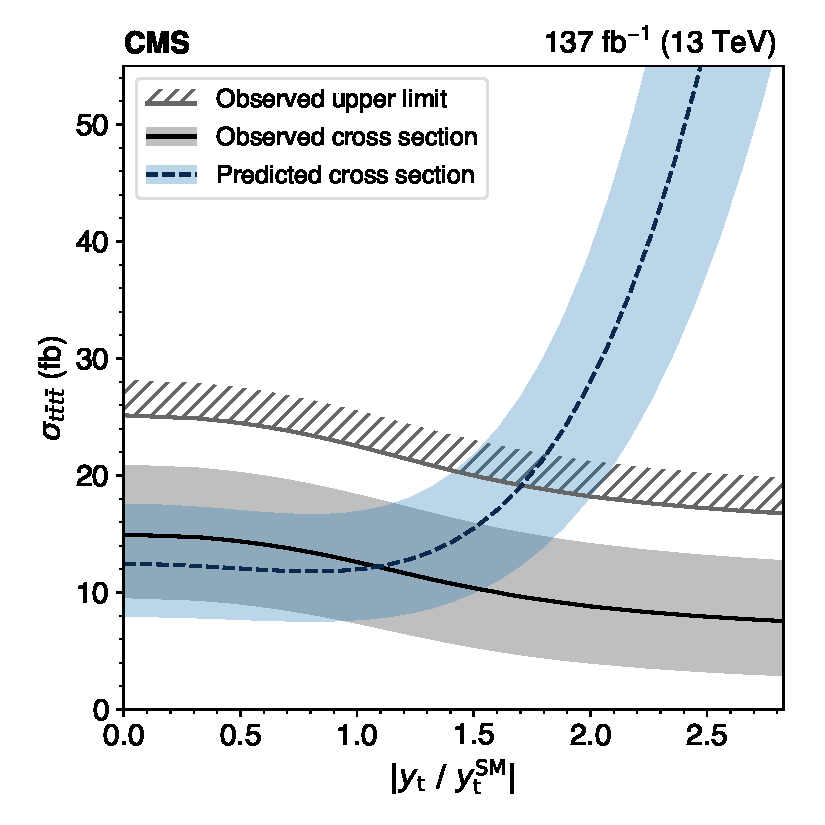
\includegraphics[width=.70\textwidth]{figs/ftp/yukawa.pdf}
\\
\caption{
    The observed \xsectttt (solid line) and 95\% \CL upper limit (hatched line) are shown as a function
    of $\abs{y_{\PQt}/y_{\PQt}^{\mathrm{SM}}}$. The predicted value (dashed line)~\cite{THEORY:TopYukawaTTTT},
    calculated at LO and scaled to the calculation from Ref.~\cite{THEORY:Frederix2017wme}, is also plotted.
    The shaded band around the measured value gives the total uncertainty, while the shaded band around
    the predicted curve shows the theoretical uncertainty associated with the renormalization and
    factorization scales.
}
\label{fig:yukawa}
\end{figure}


\FloatBarrier

\subsection{Oblique Higgs parameter}

To calculate an upper limit of $\hat{H}$, the BDT analysis is repeated
several times using simulated samples of \tttt signal events with different
values of $\hat{H}$ to account for small acceptance and kinematic
differences. During each fit, we rescale the \ttH cross section by
$(1-\hat{H})^2$ due to its $\hat{H}$ dependency. This results in the 95\% \CL
upper limit of $\hat{H} < 0.12$. For reference, using recent LHC on-shell
Higgs boson measurements, the authors of Ref.~\cite{THEORY:ObliqueHiggs2019}
obtained a constraint of $\hat{H} < 0.16$ at 95\% \CL.


\subsection{Off-shell particles}

In order to study the off-shell effect of new particles with $m < 2m_\PQt$,
we first consider neutral scalar ($\phi$) and neutral vector ($\cPZpr$)
particles that couple to top quarks. Based on simulation, these new particles
affect the signal acceptance by less than 10\%, so we recalculate the
\xsectttt upper limit of the BDT analysis including an additional 10\%
uncertainty in the acceptance, and obtain the 95\% \CL upper limit of
$23.0~\unit{fb}$ on the total \tttt cross section, slightly weaker than the
nominal limit of $22.5~\unit{fb}$. Comparing this upper limit to the predicted
cross section in models where \tttt production includes a $\phi$ or a
$\cPZpr$ in addition to SM contributions, we set limits on the masses and
couplings of these new particles, shown in
Fig.~\ref{fig:ZprimePhiExclusions}. These two-dimensional limits 
exclude couplings larger
than 1.2 for $m_{\phi}$ in the 25--340\GeV range and larger than 0.1 (0.9)
for $m_{\cPZpr} = 25$ (300)\GeV.

\begin{figure}[!hbtp]
\centering
    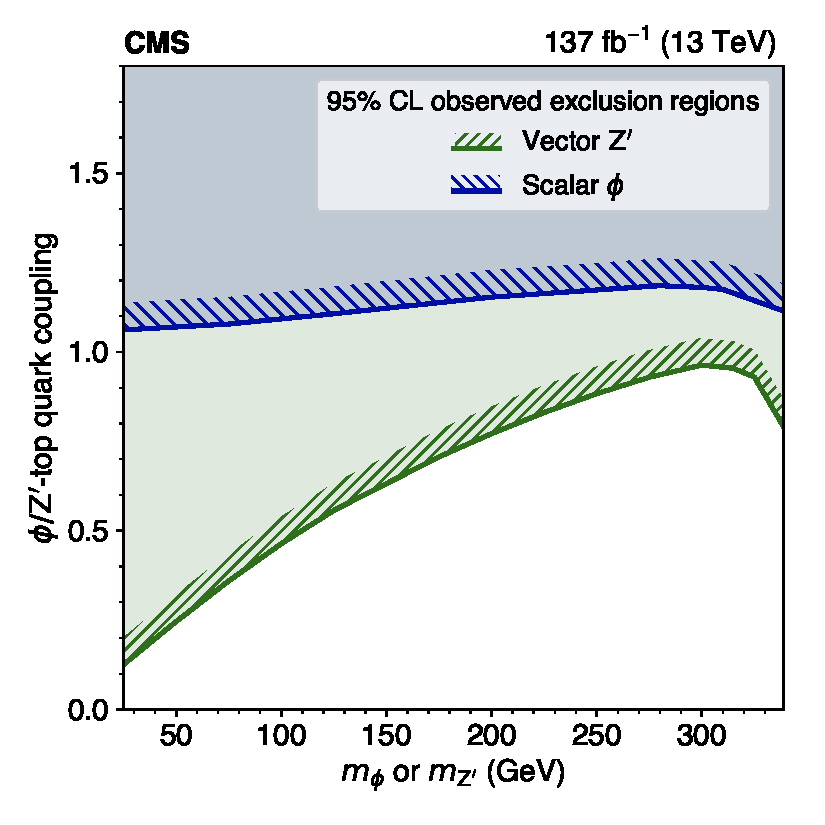
\includegraphics[width=.70\textwidth]{figs/ftp/plot_2d_phizprime.pdf}
\caption{
    The 95\% \CL exclusion regions in the plane of the $\phi/\cPZpr$-top quark coupling versus
    $m_{\phi}$ or $m_{\cPZpr}$. The excluded regions are above the hatched lines.
    }
\label{fig:ZprimePhiExclusions}
\end{figure}


\FloatBarrier

\subsection{On-shell particles}

We finally consider on-shell effects from new scalar and pseudoscalar
particles with $m > 2m_\PQt$. The production rate of these
particles in association with a single top quark ($\PQt\PQq\PH/\PSA$,
$\PQt\PW\PH/\PSA$) is significant, so we include these processes in
addition to $\PQt\overline{\PQt}\PH/\PSA$. These processes 
also do not suffer significant
interference with the SM \tttt process. To obtain upper limits on the sum of
these processes followed by the decay $\PH/\PSA\to \ttbar$, we use the BDT
analysis and treat the SM \tttt process as a background.
Figure~\ref{fig:HiggsLimits} shows excluded cross sections as a function
of the mass of the scalar and pseudoscalar particles. Comparing these
limits with the Type-II 2HDM cross sections with $\tan\beta = 1$ in the
alignment limit, we exclude scalar (pseudoscalar) masses up to 470~(550)\GeV,
which improves the limits from a previous CMS analysis~\cite{CMS:mySUS2016}
by more than 100\GeV.
Similarly, we consider a simplified model
of dark matter which includes a Dirac
fermion dark matter candidate, $\chi$, in addition to $\PH/\PSA$, and where
the couplings of $\PH/\PSA$ to SM fermions and $\chi$ are determined by
parameters $g_\mathrm{SM}$ and $g_\mathrm{DM}$, respectively. 
Exclusions similar to those from 2HDM are reached by assuming $g_\mathrm{SM}
= 1$ and $g_\mathrm{DM} = 1$, and taking $m_{\PH/\PSA} < 2 m_\chi$. 
Relaxing
the 2HDM assumption of $\tan\beta = 1$, Fig.~\ref{fig:HiggsLimitsTB} shows
the 2HDM limit as a function of $\PH/\PSA$ mass and $\tan\beta$, considering
one new particle at a time and also including a scenario with $m_\PH =
m_\PSA$. Values of $\tan\beta$ up to 0.8--1.6 are
excluded. These exclusions are comparable
to those of a recent CMS search for the resonant production of $\PH/\PSA$ in
the $\Pp\to \PH/\PSA \to \ttbar$ channel~\cite{CMS:HIG17027}. Relaxing the
$m_{\PH/\PSA} < 2 m_\chi$ assumption in the dark matter model,
we obtain
Fig.~\ref{fig:DMLimits}, which shows the limit 
as a function of the
masses of both $\PH/\PSA$ and $\chi$, for $g_\mathrm{DM} = 1$ and for two
different assumptions of $g_\mathrm{SM}$. Large sections of the phase space
are excluded, which is
is complementary to that of analyses considering invisible decays of $\PH/\PSA$
 such as in Refs.~\cite{CMS:DMsingletop, ATLAS:Aaboud2017rzf}.

\begin{figure*}[!hbtp]
\centering
    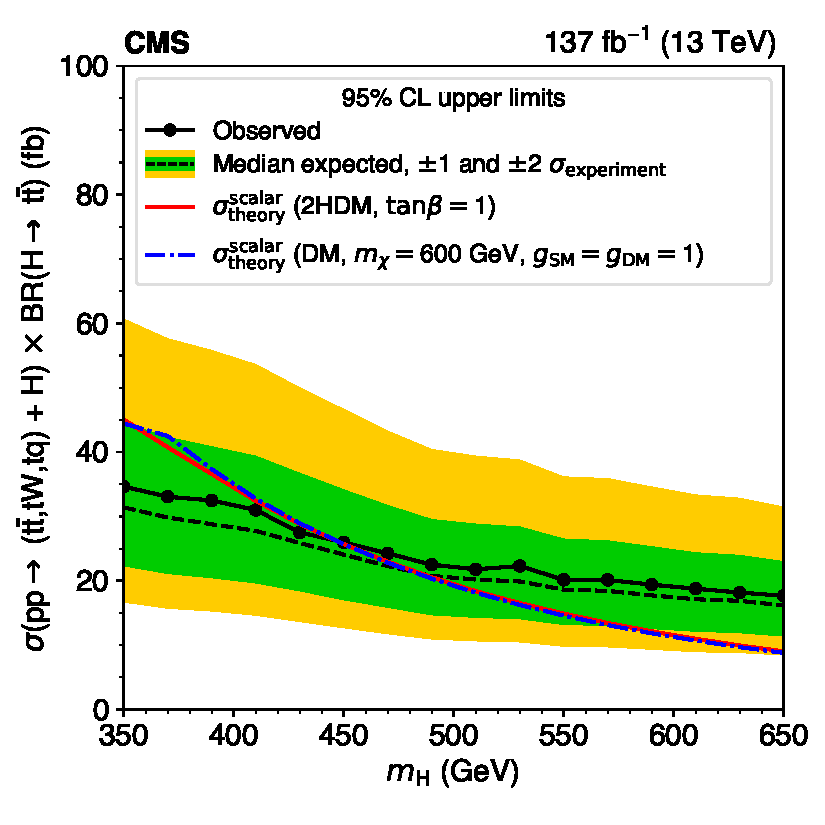
\includegraphics[width=.49\textwidth]{figs/ftp/ft_higgs_sc_scan_limit.pdf}
    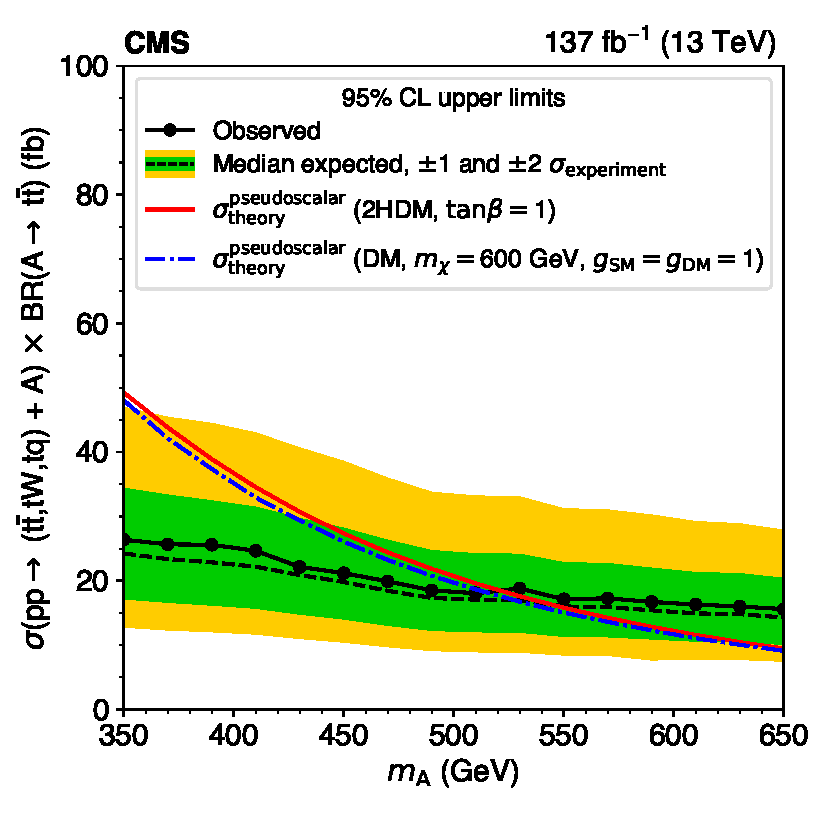
\includegraphics[width=.49\textwidth]{figs/ftp/ft_higgs_ps_scan_limit.pdf}
\caption{
    The observed (points) and expected (dashed line) 95\% \CL upper limits on the cross section
    times branching fraction to \ttbar for the production of a new heavy scalar \PH (left) and pseudoscalar \PSA (right),
    as a function of mass. The inner and outer bands around the expected limits indicate the regions containing 68 and 95\%,
    respectively, of the distribution of limits under the background-only hypothesis. Theoretical values are shown for Type-II 2HDM
    in the alignment limit (solid line) and simplified dark matter (dot-dashed line) models.
}
\label{fig:HiggsLimits}
\end{figure*}

\begin{figure*}[!hbtp]
\centering
    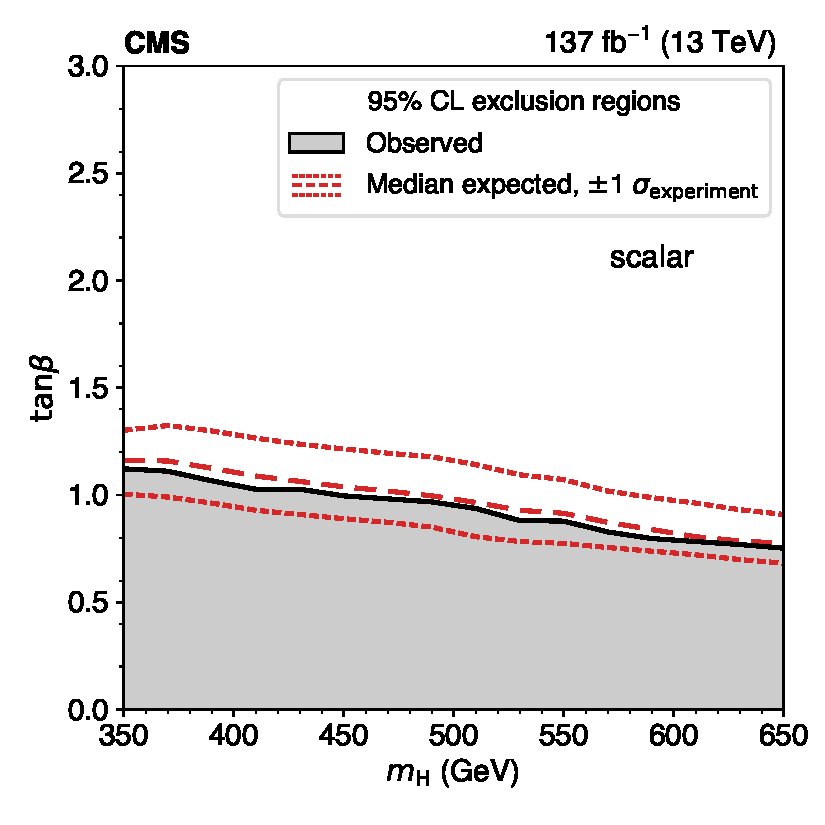
\includegraphics[width=.49\textwidth]{figs/ftp/plot_2d_2hdm_tanbetaexclusion_h.pdf}
    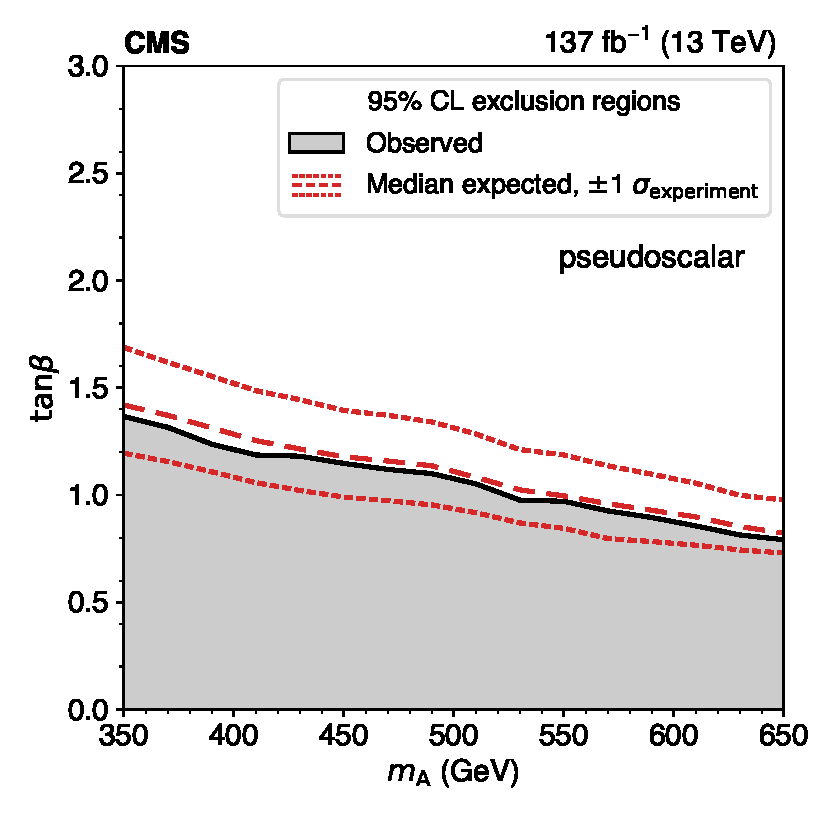
\includegraphics[width=.49\textwidth]{figs/ftp/plot_2d_2hdm_tanbetaexclusion_a.pdf}
    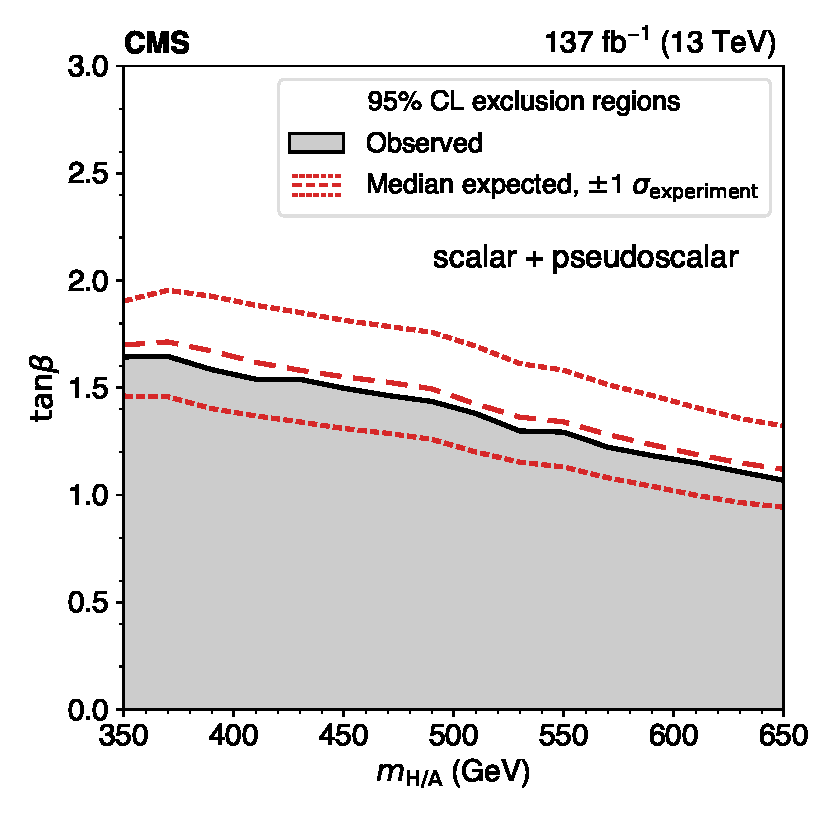
\includegraphics[width=.49\textwidth]{figs/ftp/plot_2d_2hdm_tanbetaexclusion_b.pdf}
\caption{
    The observed (solid curve) and expected (long-dashed curve) 95\% \CL exclusion regions in the $\tan\beta$ versus mass plane
    for Type-II 2HDM models in the alignment limit for a new scalar \PH (upper left), pseudoscalar \PSA (upper right), and both (lower) particles.
    The short-dashed curves around the expected limits indicate the region containing 68\% of the distribution of limits expected under the
    background-only hypothesis. The excluded regions are below the curves.
}
\label{fig:HiggsLimitsTB}
\end{figure*}

\begin{figure*}[!hbtp]
\centering
    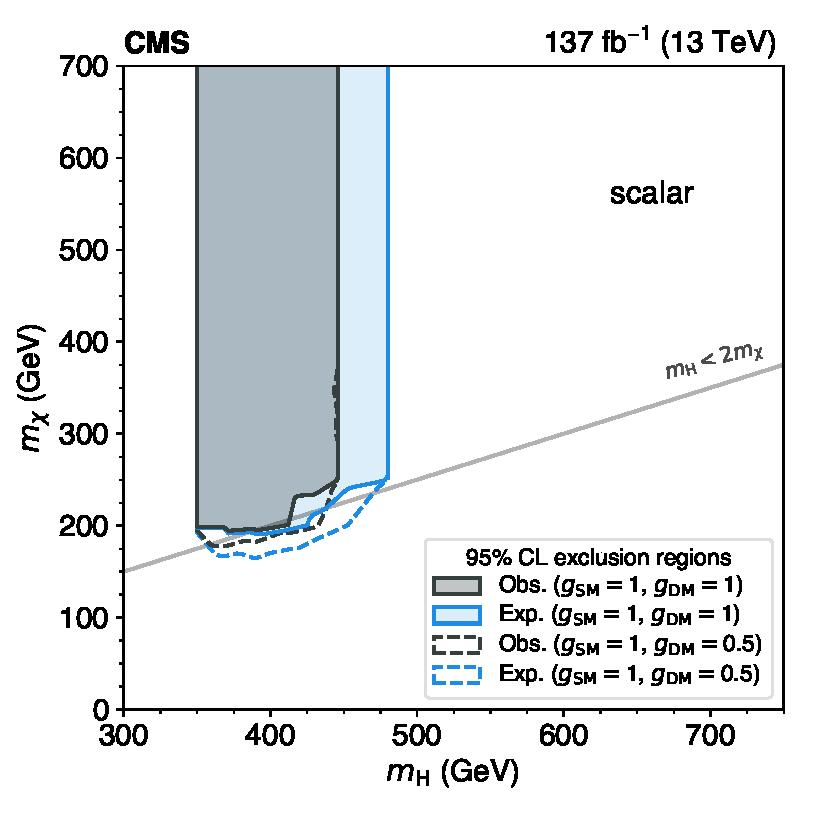
\includegraphics[width=.49\textwidth]{figs/ftp/plot_2d_dmscalar_xsec_totsm_bothcouplings.pdf}
    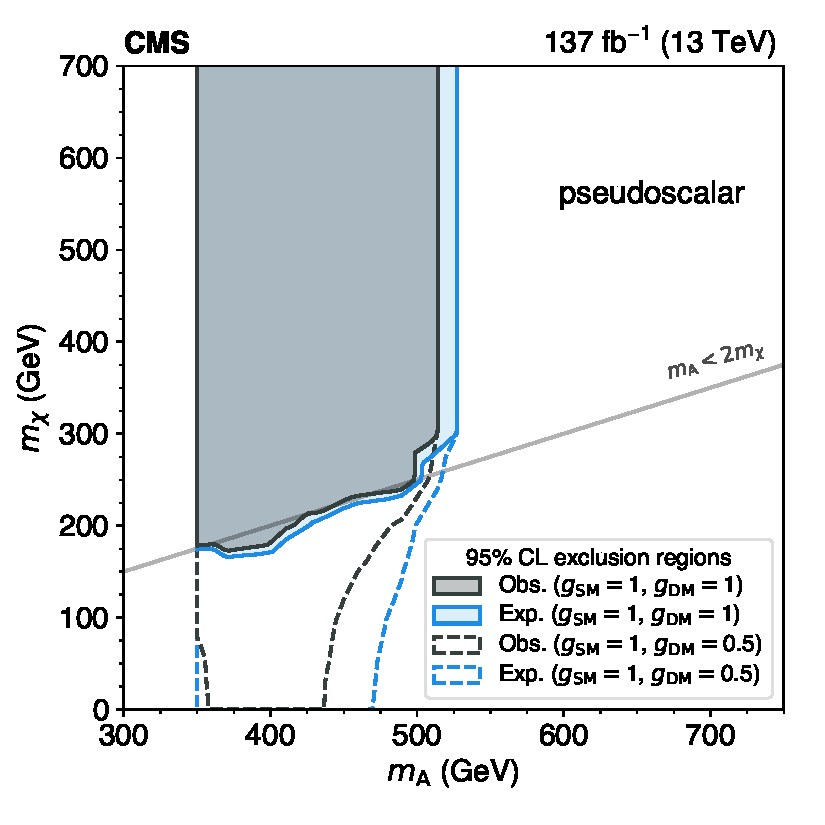
\includegraphics[width=.49\textwidth]{figs/ftp/plot_2d_dmpseudo_xsec_totsm_bothcouplings.pdf}
\caption{
	Exclusion regions at 95\% \CL in the plane of $m_\chi$ vs. $m_{\PH}$ (left) or $m_{\PSA}$ (right).
    The outer lighter and inner darker solid curves show the expected and observed limits, respectively,
    assuming $g_\mathrm{SM} = g_\mathrm{DM} = 1$. The excluded regions, shaded, are above the limit curves.
    The dashed lines show the limits assuming a weaker coupling between $\PH/\PSA$ and $\chi$, $g_\mathrm{DM} = 0.5$.
    }
\label{fig:DMLimits}
\end{figure*}

\FloatBarrier